% ===========================================================================
%
%		FEDERICO II THESIS TEMPLATE - ENGLISH
%  					* the main file
%	 
% 		AUTHOR:  		Antonio Esposito (antonio.esposito103@studenti.unina.it)
%		LAST UPDATED:	2017/06/17
%		ORIGINAL FILE:	LaTeX template of Charles University in Prague
%
% ===========================================================================

%		Single page layout:
\documentclass[12pt, a4paper]{report}
\let\openright=\clearpage

%		Double page layout
% \documentclass[12pt, a4paper, twoside, openright]{report}
% \let\openright=\cleardoublepage


%
%		Additional useful packages
%
\usepackage[T1]{fontenc}			% output font encoding
\usepackage[utf8]{inputenc}			% accented letters from keyboard
\usepackage[italian]{babel}		% document languages (the last is the main one)
\usepackage{setspace}				
\usepackage{multicol}				% multi-column layout
\usepackage{url}					% uniform resource locator
\usepackage{blindtext}
\usepackage{verbatim}
\usepackage{xcolor,colortbl}
\usepackage[hidelinks]{hyperref}
\usepackage{tabularx}
\usepackage{amsmath}        
\usepackage{amsfonts}       
\usepackage{amsthm} 
\usepackage{amssymb}      
\usepackage{pdfpages} 
\usepackage{bm}     
\usepackage{float}        
\usepackage{graphicx}       
\usepackage{psfrag}         
\usepackage{longtable}
\usepackage{fancyvrb}
\usepackage{bbding}         
\usepackage{dcolumn}        
\usepackage{booktabs}       
\usepackage{paralist}       
\usepackage{indentfirst}    
\usepackage[nottoc]{tocbibind}

\newcommand{\FIGDIR}{./Figures}    		% directory containing figures
\addto\captionsitalian{% Replace "english" with the language you use
  \renewcommand{\contentsname}%
    {Indice}%
}
%%COLORI%%
\definecolor{LightGray}{gray}{0.95}
\definecolor{Gray}{gray}{0.75}
%%%%% ------------------------------------------------------------
\DefineVerbatimEnvironment{PCinout}{Verbatim}{fontsize=\small, frame=single}

\newcommand{\R}{\mathbb{R}}
\newcommand{\N}{\mathbb{N}}

\DeclareMathOperator{\pr}{\textsf{P}}
\DeclareMathOperator{\E}{\textsf{E}\,}
\DeclareMathOperator{\var}{\textrm{var}}
\DeclareMathOperator{\sd}{\textrm{sd}}


\newcommand{\T}[1]{#1^\top}        

\newcommand{\goto}{\rightarrow}
\newcommand{\gotop}{\stackrel{P}{\longrightarrow}}
\newcommand{\maon}[1]{o(n^{#1})}
\newcommand{\abs}[1]{\left|{#1}\right|}
\newcommand{\dint}{\int_0^\tau\!\!\int_0^\tau}
\newcommand{\isqr}[1]{\frac{1}{\sqrt{#1}}}

\newcommand{\pulrad}[1]{\raisebox{1.5ex}[0pt]{#1}}
\newcommand{\mc}[1]{\multicolumn{1}{c}{#1}}


%
%
%%%	MAIN DOCUMENT
%
%

\begin{document}

% ===========================================================================
%
%		FEDERICO II THESIS TEMPLATE - ENGLISH
%  					* the header
%
%		AUTHOR:  		Antonio Esposito (antonio.esposito103@studenti.unina.it)
%		LAST UPDATED:	2017/06/20
%
% ===========================================================================

%
%%%		TITLE PAGE
%
\pagestyle{empty}
\begin{center}

% TO EDIT ACCORDINGLY TO...
% -----------------------------------------------------------------------------------------------
%

% ... University Name
{\bfseries\Huge Università degli Studi di Napoli\\}
\vspace{2.54mm}
{\bfseries\Huge Federico II\\}
\vspace{5mm}

% ... Logo
\centerline{\mbox{
\includegraphics[width=36mm]{\FIGDIR/fiilogo}}}

% ... Departement
\medskip
{\bfseries\LARGE Dipartimento di Ingegneria Elettrica e\\}
\vspace{2.54mm}
{\bfseries\LARGE delle Tecnologie dell'Informazione\\}
\vspace{2.54mm}

% ... Degree Class
{\emph{\large Classe di Laurea di Scienze e tecnologie Informatiche,\\}}
{\emph{\large Classe n. L-31\\}}
\vspace{2.54mm}

% ... Degree Course
{\large Corso di Laurea Triennale in Informatica\\}
\vspace{5mm}

% Change the name of Departement, Class and Cource in English?

%
% -----------------------------------------------------------------------------------------------
%

\vfill
{\Large Progetto\\}
\vspace{4mm}
{\emph{\LARGE Cerca Viaggi 2019\\}}		% Thesis title
\vspace{4mm}

\vfill

\begin{multicols}{2}
	{\large Docente:\\}
	Prof. Di Martino Sergio\\
	\vspace{10mm}
	\columnbreak
	{\large Candidati:\\}
	Turco Mario\\
	Matr. N86002503\\
	Longobardi Francesco\\
	Matr. N86002468\\
	Rauso Giuseppe\\
	Matr. N86002481
	\vspace{10mm}
\end{multicols}

\vfill

% Fill the year
{\large Academic Year\\ 2019/2020}

\end{center}


\pagenumbering{roman}

%
%%%		TABLE OF CONTENTS AND OTHER
%
\newpage
\openright
{\hypersetup{hidelinks}
\tableofcontents
}


%
%%%		Optional
%

%\listoffigures
%\listoftables

%\chapter*{List of abbreviations}
%\addcontentsline{toc}{chapter}{List of abbreviations}


\pagenumbering{arabic}
% ===========================================================================
%
%		FEDERICO II THESIS TEMPLATE - ENGLISH
%  					* an example of Introduction
%	 
% 		AUTHOR:  		Antonio Esposito (antonio.esposito103@studenti.unina.it)
%		LAST UPDATED:	2017/06/20
%
% ===========================================================================

\chapter*{Introduction}
\addcontentsline{toc}{chapter}{Introduction}

The introduction is prior to any chapter. 
It has to present the problem taken into exam and clarify the aim of the work, eventually pointing out the original contributions to the scientific literature; the introduction can cointain a brief summary of the thesis organization. The following chapters include the description of the state of the art concerning the discussed topic. For experimental theses, some chapters are dedicated to the description of the innovative solution and its validation. The conclusions, finally, must sum up briefly the faced challenges and report the main consideration that can be done after the experimental results.

The manuscript must include a bibliography that lists all the references (books, scientific articles, theses, web sites, etc.), together with proper information about where the reader can find the cited material. See the references of this file to understand the desired format for the citations.

In the following part of this file, more details on the preparation and presentation of the thesis are given in Chapter 1. Then, examples of typesetting of mathematical text are shown in Chapter 2. Table, figue, and software code are instead discussed in Chapter 3. Conclusions follow. The aim of the present file is to show an example of thesis structure, and, in its \LaTeX version, the main commands that can be useful during a thesis writing are used: in this way, the student that is willing to write his/her thesis with \LaTeX, has a good starting point. It's worth noting that the current version of the file was written by an italian student, and this means that lots of errors are present, expecially regarding the english grammar\dots

%Revisioni
\part{Documento dei Requisiti Software}
% ===========================================================================
%
%		FEDERICO II THESIS TEMPLATE - ENGLISH
%  					* an example of Chapter 1: information about the discussion of the thesis
%	 
% 		AUTHOR:  		Antonio Esposito (antonio.esposito103@studenti.unina.it)
%		LAST UPDATED:	2017/06/20
%
% ===========================================================================

\chapter{Modello funzionale}

This chapter contains useful information for the preparation and the presentation of the master degree thesis for students of Electronic Engineering (M61), at the University of Study of Naples Federico II.

The final test for the Master Degree course in Electronic Engineering consists in the preparation and discussion of a thesis, written with the help of a supervisor (eventually with one or two co-supervisors). This work is the final result of the student career and it testifies his/her ability in exploring in deep the topics encountered during the degree course.

%%%%% ===============================================================================
\section{Modellazione dei casi d'uso}

The supervisor is one of the professors that the candidate encountered during the degree course. Usually, the student finds its supervisor through informal talks, once provided that the professor is available and the student is interested in the professor's topics of interest. The degree course, on its website \url{www.ingegneria-elettronica.unina.it}, has defined a page with a non-esaustive list of available theses topics, in order to facilitate the information exchange between students and professors.

In case the thesis is developed after an intra-moenia internship, among one of the laboratories of the departement, the tutor that has already followed the student during the internship becomes the supervisor.

The supervisor defines the thesis topic. As already mentioned, the supervisor can be helped by one (or two maximum) co-supervisor. Supervisor and co-supervisor must guide and assist the student during the thesis developement and also provide him all the needed methodological and practical instruments. During the thesis are usually foreseen periodical meetings of the candidate with the supervisor, during which the ongoing work and the obtained results are discussed, also to define the future steps of the work.


%%%%% ===============================================================================
\section{Tabelle di Cockburn}
Di seguito si riportano, divise per attori, le tabelle di Cockburn relative agli Use Case Diagram.
\subsection{Amministratore}

\begin{table}[h!]    
\def\arraystretch{1.5}
\caption{L'amministratore effettua il login }

%Intestazione tabella%
\begin{tabularx}{\textwidth}{|l|X|X|X|X|}
 \rowcolor{Gray}
  \hline Use Case \#1 & \multicolumn{4} {l|}{Effettua Login} \\ \hline Goal in
  Context & \multicolumn{4}{>{\hsize=\dimexpr 4\hsize+4\tabcolsep+2\arrayrulewidth\relax}X|}{%
    L'amministratore vuole accedere all'applicativo di Back-Office} \\
 \hline Preconditions & \multicolumn{4}{>{\hsize=\dimexpr 4\hsize+4\tabcolsep+2\arrayrulewidth\relax}X|}{%
 L'amministratore non ha effettuto lo use case "Effettua Login".  } \\
 \hline Success End Conditions &
 \multicolumn{4}{>{\hsize=\dimexpr 4\hsize+4\tabcolsep+2\arrayrulewidth\relax}X|}{ Il login dell'amministratore va a buon fine.} \\
 \hline Failed End Conditions &
 \multicolumn{4}{>{\hsize=\dimexpr 4\hsize+4\tabcolsep+2\arrayrulewidth\relax}X|}{I dati di login sono errati o il server non è raggiungibile.} \\
 \hline Primary Actor &
  \multicolumn{4}{l|}{Amministratore} \\
 \hline Trigger & 
 \multicolumn{4}{>{\hsize=\dimexpr 4\hsize+4\tabcolsep+2\arrayrulewidth\relax}X|}{L'amministratore preme il pulsante "Login" nella schermata LoginForm visibile all'avvio del software.} \\
\hline
%Main Scenario%
\multicolumn{5}{|>{\hsize=\dimexpr 4\hsize+4\tabcolsep+2\arrayrulewidth\relax}c|}{Main Scenario}\\\hline
\end{tabularx}
\setlength{\tabcolsep}{8pt}
\renewcommand{\arraystretch}{1.5}
    \begin{tabularx}{\textwidth}{|c|X|X|}
        Step\# & Amministratore & Sistema \\
        \hline
         1 &Compila correttamente i textField Username e Password  & \\
         \hline
         2 &Preme il pulsante "Login" dalla schermata LoginForm  & \\
         \hline
         3 &  &Mostra schermata HomePage\\
        \hline
    \end{tabularx} 
    \end{table}
    \begin{table}[H]
        \caption{Effettua Login - Estensione 1}
    %Extension 1%
    \begin{tabularx}{\textwidth}{|c|X|X|}
            \hline
            \rowcolor{LightGray}
            \multicolumn{3}{|>{\hsize=\dimexpr 4\hsize+4\tabcolsep+2\arrayrulewidth\relax}c|}{Extension 1: l'amministatore inserisce dati errati}\\\hline
            Step\# & Amministratore & Sistema \\
            \hline
             1 a &  Non complia o compila erroneamente i textField Username e Password& \\
             \hline
             2 a & Preme il pulsante Login & \\
             \hline
             3 a & & Mostra CredenzialiErrateDialog \\
             \hline
             4 a & Preme il tasto Ok&  \\
             \hline
             5 a & & Mostra LoginForm e termina caso d'uso\\
             \hline        
        \end{tabularx} 
    \end{table}
    \begin{table}[h!]
        \caption{Effettua Login - Estensione 2}
    %Extension 2%
    \begin{tabularx}{\textwidth}{|c|X|X|}
        \hline
        \rowcolor{LightGray}
        \multicolumn{3}{|>{\hsize=\dimexpr 4\hsize+4\tabcolsep+2\arrayrulewidth\relax}c|}{Extension 2: il server non è raggiungibile}\\\hline
        Step\# & Amministratore & Sistema \\
        \hline
         1 b &  Compila i campi username e password& \\
         \hline
         2 b & Preme il pulsante Login & \\
         \hline
         3 a & & Mostra 'Connessione assente dialog' e termina caso d'uso \\
         \hline
       
    \end{tabularx} 
\end{table}


\begin{table}[H]    
\def\arraystretch{1.5}
\caption{L'amministratore valuta una recensione}

%Intestazione tabella%
\begin{tabularx}{\textwidth}{|l|X|X|X|X|}
  \rowcolor{Gray}
  \hline Use Case \#2 & \multicolumn{4} {l|}{Valuta Recensione} \\ \hline Goal in
  Context & \multicolumn{4}{>{\hsize=\dimexpr 4\hsize+4\tabcolsep+2\arrayrulewidth\relax}X|}{%
    L'amministratore valuta una recensione.} \\
 \hline Preconditions & \multicolumn{4}{>{\hsize=\dimexpr 4\hsize+4\tabcolsep+2\arrayrulewidth\relax}X|}{%
 L'amministratore ha effettuto lo use case "Effettua Login".  } \\
 \hline Success End Conditions &
 \multicolumn{4}{>{\hsize=\dimexpr 4\hsize+4\tabcolsep+2\arrayrulewidth\relax}X|}{ L'amministratore valuta una recensione. Il sistema tiene traccia di tale operazione.} \\
 \hline Failed End Conditions &
 \multicolumn{4}{>{\hsize=\dimexpr 4\hsize+4\tabcolsep+2\arrayrulewidth\relax}X|}{L'amministatore preme annulla. L'amministrazione valuta una recensione che è già stata valutata. Il server non è raggiungibile.} \\
 \hline Primary Actor &
  \multicolumn{4}{l|}{Amministratore} \\
 \hline Trigger & 
 \multicolumn{4}{>{\hsize=\dimexpr 4\hsize+4\tabcolsep+2\arrayrulewidth\relax}X|}{L'amministratore preme il pulsante "Recensioni" nella Homepage.} \\
\hline
%Main Scenario%
\multicolumn{5}{|>{\hsize=\dimexpr 4\hsize+4\tabcolsep+2\arrayrulewidth\relax}c|}{Main Scenario}\\\hline
\end{tabularx}
\setlength{\tabcolsep}{8pt}
\renewcommand{\arraystretch}{1.5}
    \begin{tabularx}{\textwidth}{|c|X|X|}
        Step\# & Amministratore & Sistema \\
        \hline
         1 &Preme il pulsante "Recensioni" nella schermata principale & \\
         \hline
         2 & & Mostra schermata "Recensioni"\\
         \hline
         3 & Clicca sulla card di una recensione  &\\
         \hline
         4 & & Mostra schermata "Visualizza Recensione"\\
       \hline
         5 & Clicca sul pulsante Accetta &\\
        \hline
        6& &Mostra 'Recensione Approvata Dialog' e termina lo use case\\
        \hline
    \end{tabularx}
    %Subvariation 1%
\end{table}
\begin{table}[h!]
    \caption{Valuta una recensione - Subvariation 1}
        \begin{tabularx}{\textwidth}{|c|X|X|}
            \hline
            \rowcolor{LightGray}
            \multicolumn{3}{|>{\hsize=\dimexpr 4\hsize+4\tabcolsep+2\arrayrulewidth\relax}c|}{Subvariation 1: l'amministatore rifiuta una recensione}\\\hline
            Step\# & Amministratore & Sistema \\
            \hline
             5 i &Preme il pulsante "Rifiuta". & \\
             \hline
             6 i & & Mostra 'Recensione Rifiutata Dialog' e termina lo use case.\\
            \hline
        \end{tabularx}
\setlength{\tabcolsep}{8pt}
\renewcommand{\arraystretch}{1.5}
\end{table}

 %Extension 1%
\begin{table}[h!]
    \caption{Valuta una recensione - Estensione 1}
    \begin{tabularx}{\textwidth}{|c|X|X|}
        \hline
        \rowcolor{LightGray}
        \multicolumn{3}{|>{\hsize=\dimexpr 4\hsize+4\tabcolsep+2\arrayrulewidth\relax}c|}{Extension 1: l'amministatore preme annulla}\\\hline
        Step\# & Amministratore & Sistema \\
        \hline
         3/5 a &Preme il pulsante "Recensioni" dal menu laterale sinistro & \\
         \hline
         4/6 a & & Ritorna alla schermata principale e termina il caso d'uso.\\
        \hline
    \end{tabularx}
\end{table}
%Estensione 2
\begin{table}[h!]
    \caption{Valuta una recensione - Estensione 2}
     \begin{tabularx}{\textwidth}{|c|X|X|}
        \hline
        \rowcolor{LightGray}
        \multicolumn{3}{|>{\hsize=\dimexpr 4\hsize+4\tabcolsep+2\arrayrulewidth\relax}c|}{Extension 2: la recensione è già stata valutata }\\\hline
         Step\# & Amministratore & Sistema \\
         \hline
          4 b  & & Mostra Fallimento Dialog e termina caso d'uso \\
          \hline
     \end{tabularx}
\end{table}
%Estensione 3
\begin{table}[h!]
    \caption{Valuta una recensione - Estensione 3}
     \begin{tabularx}{\textwidth}{|c|X|X|}
        \hline
        \rowcolor{LightGray}
        \multicolumn{3}{|>{\hsize=\dimexpr 4\hsize+4\tabcolsep+2\arrayrulewidth\relax}c|}{Extension 3: il server non è raggiungibile }\\\hline
         Step\# & Amministratore & Sistema \\
         \hline
          4/6 c  & & Mostra Connessione Assente Dialog e termina caso d'uso \\
          \hline
     \end{tabularx}
\end{table}
\pagebreak
\subsection{Utente non autenticato}

%Intestazione tabella%
\begin{table}
\begin{tabularx}{\textwidth}{|l|X|X|X|X|}
  \hline Use Case \#1 & \multicolumn{4} {l|}{Utente effettua Login} \\ \hline Goal in
  Context & \multicolumn{4}{>{\hsize=\dimexpr 4\hsize+4\tabcolsep+2\arrayrulewidth\relax}X|}{%
    L'utente non loggato effettua il login} \\
 \hline Preconditions & \multicolumn{4}{>{\hsize=\dimexpr 4\hsize+4\tabcolsep+2\arrayrulewidth\relax}X|}{%
 L'utente non autenticato non ha effettuto lo use case "Utente effettua Login".  } \\
 \hline Success End Conditions &
 \multicolumn{4}{>{\hsize=\dimexpr 4\hsize+4\tabcolsep+2\arrayrulewidth\relax}X|}{ Il login dell'utente va a buon fine.} \\
 \hline Failed End Conditions &
 \multicolumn{4}{>{\hsize=\dimexpr 4\hsize+4\tabcolsep+2\arrayrulewidth\relax}X|}{I dati di login sono errati oppure il server non è raggiungibile.} \\
 \hline Primary Actor &
  \multicolumn{4}{l|}{Utente non loggato} \\
 \hline Trigger & 
 \multicolumn{4}{>{\hsize=\dimexpr 4\hsize+4\tabcolsep+2\arrayrulewidth\relax}X|}{L'utente preme il pulsante 'Login' nel Navigation Drawer laterale dalla schermata 'HomePage utente non loggato'.} \\
\hline
%Main Scenario%
\multicolumn{5}{|>{\hsize=\dimexpr 4\hsize+4\tabcolsep+2\arrayrulewidth\relax}c|}{Main Scenario}\\\hline
\end{tabularx}
\setlength{\tabcolsep}{8pt}
\renewcommand{\arraystretch}{1.5}
    \begin{tabularx}{\textwidth}{|c|X|X|}
        Step\# & Utente & Sistema \\
        \hline
         1 &Compila correttamente i textField Username e Password  & \\
         \hline
         2 &Preme il pulsante "Login" dalla schermata LoginForm  & \\
         \hline
         3 &  &Mostra schermata HomePage\\
        \hline
    \end{tabularx}
    %Extension 1%
        \begin{tabularx}{\textwidth}{|c|X|X|}
            \hline
            \multicolumn{3}{|>{\hsize=\dimexpr 4\hsize+4\tabcolsep+2\arrayrulewidth\relax}c|}{Extension 1: l'utente inserisce dati errati}\\\hline
            Step\# & Utente & Sistema \\
            \hline
             1 a &  Compila erroneamente i textField Username e Password& \\
             \hline
             2 a & Preme il pulsante Login & \\
             \hline
             3 a & & Mostra schermata Login Dati Errati Dialog \\
             \hline
             4 a & Preme il tasto 'Riprova'&  \\
             \hline
             5 a & & Mostra Login e termina caso d'uso\\
             \hline        
        \end{tabularx} 
    %Extension 2%
    \begin{tabularx}{\textwidth}{|c|X|X|}
      \hline
      \multicolumn{3}{|>{\hsize=\dimexpr 4\hsize+4\tabcolsep+2\arrayrulewidth\relax}c|}{Extension 2: l'utente non compila tutti i campi}\\\hline
      Step\# & Utente & Sistema \\
      \hline
       1 b &  Non compila o compila solo un tra i textField Username e Password& \\
       \hline
       2 b & Preme il pulsante Login & \\
       \hline
       3 b & & Mostra schermata Login campi vuoti Dialog \\
       \hline
       4 b & Preme il tasto 'Riprova'&  \\
       \hline
       5 b & & Mostra Login e termina caso d'uso\\
       \hline        
  \end{tabularx}
\end{table}
\pagebreak
%Extension 3%
\begin{table}
\begin{tabularx}{\textwidth}{|c|X|X|}
  \hline
  \multicolumn{3}{|>{\hsize=\dimexpr 4\hsize+4\tabcolsep+2\arrayrulewidth\relax}c|}{Extension 3: il server risulta non raggiungibile}\\\hline
  Step\# & Utente & Sistema \\
  \hline
   3 c & & Mostra schermata Login server irraggiungibile \\
   \hline
   4 c & Preme il tasto 'Riprova'&  \\
   \hline
   5 c & & Mostra Login e termina caso d'uso\\
   \hline        
\end{tabularx} 
\end{table}


%Intestazione tabella%
\begin{table}[h!]
\caption{L'utente non loggato effettua la registazione}
\begin{tabularx}{\textwidth}{|l|X|X|X|X|}
  \hline Use Case \#2 & \multicolumn{4} {l|}{L'utente non loggato si registra alla piattaforma} \\ \hline Goal in
  Context & \multicolumn{4}{>{\hsize=\dimexpr 4\hsize+4\tabcolsep+2\arrayrulewidth\relax}X|}{%
    L'utente non loggato effettua la registrazione} \\
 \hline Preconditions & \multicolumn{4}{>{\hsize=\dimexpr 4\hsize+4\tabcolsep+2\arrayrulewidth\relax}X|}{%
 -  } \\
 \hline Success End Conditions &
 \multicolumn{4}{>{\hsize=\dimexpr 4\hsize+4\tabcolsep+2\arrayrulewidth\relax}X|}{ La registrazione dell'utente va a buon fine.} \\
 \hline Failed End Conditions &
 \multicolumn{4}{>{\hsize=\dimexpr 4\hsize+4\tabcolsep+2\arrayrulewidth\relax}X|}{Il server non è raggiungibile o l'utente immette dati non validi.} \\
 \hline Primary Actor &
  \multicolumn{4}{l|}{Utente non loggato} \\
 \hline Trigger & 
 \multicolumn{4}{>{\hsize=\dimexpr 4\hsize+4\tabcolsep+2\arrayrulewidth\relax}X|}{L'utente preme il pulsante 'Registrati' nel Navigation Drawer laterale dalla schermata 'HomePage utente non loggato'.} \\
\hline
%Main Scenario%
\multicolumn{5}{|>{\hsize=\dimexpr 4\hsize+4\tabcolsep+2\arrayrulewidth\relax}c|}{Main Scenario}\\\hline
\end{tabularx}
\setlength{\tabcolsep}{8pt}
\renewcommand{\arraystretch}{1.5}
    \begin{tabularx}{\textwidth}{|c|X|X|}
        Step\# & Utente & Sistema \\
        \hline
         1 &Compila correttamente tutti i textField ed il date picker  & \\
         \hline
         2 &Preme il pulsante "Fine" dalla schermata Registrazione  & \\
         \hline
         3 &  &Mostra schermata "Registrazione success dialog" e termina il caso d'uso\\
        \hline
    \end{tabularx}
  \end{table}
  \begin{table}[h!]
    \caption{Effettua registrazione - Estensione 1}
    %Extension 1%
        \begin{tabularx}{\textwidth}{|c|X|X|}
            \hline
            \multicolumn{3}{|>{\hsize=\dimexpr 4\hsize+4\tabcolsep+2\arrayrulewidth\relax}c|}{Extension 1: l'utente inserisce dati di un utente già registrato}\\\hline
            Step\# & Utente & Sistema \\
            \hline
             1 a &  Compila i textField inserendo i dati di un account già registrato& \\
             \hline
             2 a & Preme il pulsante "Fine" & \\
             \hline
             3 a & & Mostra schermata "Registrazione utente esistente fail dialog" e termina il caso d'uso\\
             \hline        
        \end{tabularx} 
      \end{table}

    %Extension 2%
    \begin{table}[h!]
    \caption{Effettura registrazione - Estensione 2}
    \begin{tabularx}{\textwidth}{|c|X|X|}
      \hline
      \multicolumn{3}{|>{\hsize=\dimexpr 4\hsize+4\tabcolsep+2\arrayrulewidth\relax}c|}{Extension 2: l'utente non compila tutti i campi o li compila in modo errato}\\\hline
      Step\# & Utente & Sistema \\
      \hline
       1 b &  Non compila o compila erroneamente i textfiel ed il datepicker& \\
       \hline
       2 b & Preme il pulsante "Fine" & \\
       \hline
       3 b & & Mostra schermata "Campi non compilato o errati dialog" e termina caso d'uso  \\
       \hline        
  \end{tabularx}
\end{table}

%Extension 3%
\begin{table}[h!]
  \caption{Effettura registrazione - Estensione 3}
\begin{tabularx}{\textwidth}{|c|X|X|}
  \hline
  \multicolumn{3}{|>{\hsize=\dimexpr 4\hsize+4\tabcolsep+2\arrayrulewidth\relax}c|}{Extension 3: il server risulta non raggiungibile}\\\hline
  Step\# & Utente & Sistema \\
  \hline
  1 c & Compila correttamente tutti i campi della registrazione&  \\
  \hline
  2 c & Preme il tasto "Fine"&  \\
  \hline
  3 c & & Mostra schermata "Registrazione server irraggiungibile" e termina caso d'uso \\
   \hline
\end{tabularx} 
\end{table}


%Intestazione tabella%
\begin{table}[H]
    \caption{L'utente non loggato visulizza una struttura}
    \begin{tabularx}{\textwidth}{|l|X|X|X|X|}
      \hline Use Case \#3 & \multicolumn{4} {l|}{L'utente non loggato visulizza una struttura} \\ \hline Goal in
      Context & \multicolumn{4}{>{\hsize=\dimexpr 4\hsize+4\tabcolsep+2\arrayrulewidth\relax}X|}{%
        L'utente non loggato visulizza una struttura} \\
     \hline Preconditions & \multicolumn{4}{>{\hsize=\dimexpr 4\hsize+4\tabcolsep+2\arrayrulewidth\relax}X|}{%
     L'Utente ha effettuato una ricerca e si trova nella schermata "Lista Strutture" } \\
     \hline Success End Conditions &
     \multicolumn{4}{>{\hsize=\dimexpr 4\hsize+4\tabcolsep+2\arrayrulewidth\relax}X|}{ L'utente visualizza i dettagli di una struttura} \\
     \hline Failed End Conditions &
     \multicolumn{4}{>{\hsize=\dimexpr 4\hsize+4\tabcolsep+2\arrayrulewidth\relax}X|}{Il server non è raggiungibile } \\
     \hline Primary Actor &
      \multicolumn{4}{l|}{Utente non loggato} \\
     \hline Trigger & 
     \multicolumn{4}{>{\hsize=\dimexpr 4\hsize+4\tabcolsep+2\arrayrulewidth\relax}X|}{} \\
    \hline
    %Main Scenario%
    \multicolumn{5}{|>{\hsize=\dimexpr 4\hsize+4\tabcolsep+2\arrayrulewidth\relax}c|}{Main Scenario}\\\hline
    \end{tabularx}
    \setlength{\tabcolsep}{8pt}
    \renewcommand{\arraystretch}{1.5}
        \begin{tabularx}{\textwidth}{|c|X|X|}
            Step\# & Utente & Sistema \\
            \hline
             1 & L'utente clicca la Card di una struttura dalla schermata "Lista Strutture"'. & \\
             \hline
             2 && Mostra la schermata "Pagina Struttura utente non loggato" e termina caso d'uso\\
             \hline
            
        \end{tabularx}
    \end{table}
    \begin{table}[H]
    \caption{Visualizza struttura - Estensione 1}
    %Extension 1%
         \begin{tabularx}{\textwidth}{|c|X|X|}
                \hline
                \multicolumn{3}{|>{\hsize=\dimexpr 4\hsize+4\tabcolsep+2\arrayrulewidth\relax}c|}{Extension 1: il server non è raggiungibile}\\\hline
                Step\# & Utente & Sistema \\
                \hline
                 2 a &  & Mostra schermata "Connessione assente" e termina caso d'uso\\
                 \hline 
        \end{tabularx} 
\end{table}
    
       


%Intestazione tabella%
\begin{table}[H]
    \caption{L'utente non loggato visulizza i dettagli di una recensione}
    \begin{tabularx}{\textwidth}{|l|X|X|X|X|}
      \hline 
      Use Case \#3 & \multicolumn{4} {l|}{L'utente non loggato visulizza i dettagli di una recensione} \\ \hline Goal in
      Context & \multicolumn{4}{>{\hsize=\dimexpr 4\hsize+4\tabcolsep+2\arrayrulewidth\relax}X|}
      {L'utente non loggato visulizza i dettagli di una recensione} \\
     \hline Preconditions & \multicolumn{4}{>{\hsize=\dimexpr 4\hsize+4\tabcolsep+2\arrayrulewidth\relax}X|}{%
     L'Utente si trova nella schermata "Pagina Struttura" avendo effettuato il caso d'uso "Visualizza una struttura } \\
     \hline Success End Conditions &
     \multicolumn{4}{>{\hsize=\dimexpr 4\hsize+4\tabcolsep+2\arrayrulewidth\relax}X|}{ L'utente visualizza i dettagli di una recensione} \\
     \hline Failed End Conditions &
     \multicolumn{4}{>{\hsize=\dimexpr 4\hsize+4\tabcolsep+2\arrayrulewidth\relax}X|}{Il server non è raggiungibile } \\
     \hline Primary Actor &
      \multicolumn{4}{l|}{Utente non loggato} \\
     \hline Trigger & 
     \multicolumn{4}{>{\hsize=\dimexpr 4\hsize+4\tabcolsep+2\arrayrulewidth\relax}X|}{} \\
    \hline
    %Main Scenario%
    \multicolumn{5}{|>{\hsize=\dimexpr 4\hsize+4\tabcolsep+2\arrayrulewidth\relax}c|}{Main Scenario}\\
    \hline
\end{tabularx}
    \setlength{\tabcolsep}{8pt}
    \renewcommand{\arraystretch}{1.5}
        \begin{tabularx}{\textwidth}{|c|X|X|}
            Step\# & Utente & Sistema \\
            \hline
             1 & Clicca la Card di una recensione dalla schermata "Pagina struttura"'. & \\
             \hline
             2 & & Mostra la schermata "Pagina Recensione" e termina caso d'uso\\
             \hline
        \end{tabularx}
   \end{table}
    \begin{table}[H]
    \caption{Visualizza struttura - Estensione 1}
    %Extension 1%
         \begin{tabularx}{\textwidth}{|c|X|X|}
                \hline
                \multicolumn{3}{|>{\hsize=\dimexpr 4\hsize+4\tabcolsep+2\arrayrulewidth\relax}c|}{Extension 1: il server non è raggiungibile}\\\hline
                Step\# & Utente & Sistema \\
                \hline
                 2 a &  & Mostra schermata "Connessione assente" e termina caso d'uso\\
                 \hline 
        \end{tabularx} 
\end{table}
    
       


\subsection{Utente autenticato}

%Intestazione tabella%
\begin{table}[H]
    \caption{L'utente non loggato visulizza una struttura}
    \begin{tabularx}{\textwidth}{|l|X|X|X|X|}
      \hline Use Case \#3 & \multicolumn{4} {l|}{L'utente non loggato visulizza una struttura} \\ \hline Goal in
      Context & \multicolumn{4}{>{\hsize=\dimexpr 4\hsize+4\tabcolsep+2\arrayrulewidth\relax}X|}{%
        L'utente non loggato visulizza una struttura} \\
     \hline Preconditions & \multicolumn{4}{>{\hsize=\dimexpr 4\hsize+4\tabcolsep+2\arrayrulewidth\relax}X|}{%
     L'Utente ha effettuato una ricerca e si trova nella schermata "Lista Strutture" } \\
     \hline Success End Conditions &
     \multicolumn{4}{>{\hsize=\dimexpr 4\hsize+4\tabcolsep+2\arrayrulewidth\relax}X|}{ L'utente visualizza i dettagli di una struttura} \\
     \hline Failed End Conditions &
     \multicolumn{4}{>{\hsize=\dimexpr 4\hsize+4\tabcolsep+2\arrayrulewidth\relax}X|}{Il server non è raggiungibile } \\
     \hline Primary Actor &
      \multicolumn{4}{l|}{Utente non loggato} \\
     \hline Trigger & 
     \multicolumn{4}{>{\hsize=\dimexpr 4\hsize+4\tabcolsep+2\arrayrulewidth\relax}X|}{} \\
    \hline
    %Main Scenario%
    \multicolumn{5}{|>{\hsize=\dimexpr 4\hsize+4\tabcolsep+2\arrayrulewidth\relax}c|}{Main Scenario}\\\hline
    \end{tabularx}
    \setlength{\tabcolsep}{8pt}
    \renewcommand{\arraystretch}{1.5}
        \begin{tabularx}{\textwidth}{|c|X|X|}
            Step\# & Utente & Sistema \\
            \hline
             1 & L'utente clicca la Card di una struttura dalla schermata "Lista Strutture"'. & \\
             \hline
             2 && Mostra la schermata "Pagina Struttura utente non loggato" e termina caso d'uso\\
             \hline
            
        \end{tabularx}
    \end{table}
    \begin{table}[H]
    \caption{Visualizza struttura - Estensione 1}
    %Extension 1%
         \begin{tabularx}{\textwidth}{|c|X|X|}
                \hline
                \multicolumn{3}{|>{\hsize=\dimexpr 4\hsize+4\tabcolsep+2\arrayrulewidth\relax}c|}{Extension 1: il server non è raggiungibile}\\\hline
                Step\# & Utente & Sistema \\
                \hline
                 2 a &  & Mostra schermata "Connessione assente" e termina caso d'uso\\
                 \hline 
        \end{tabularx} 
\end{table}
    
       


%Intestazione tabella%
\begin{table}[H]
    \caption{L'utente loggato aggiunge una recensione}
    \begin{tabularx}{\textwidth}{|l|X|X|X|X|}
      \hline Use Case \#3 & \multicolumn{4} {l|}{L'utente loggato aggiunge una recensione} \\ \hline Goal in
      Context & \multicolumn{4}{>{\hsize=\dimexpr 4\hsize+4\tabcolsep+2\arrayrulewidth\relax}X|}{%
        L'utente loggato aggiunge con successo una recensione} \\
     \hline Preconditions & \multicolumn{4}{>{\hsize=\dimexpr 4\hsize+4\tabcolsep+2\arrayrulewidth\relax}X|}{%
     L'Utente si trova nella schermata "Pagina Struttura" dopo aver effettuato il caso d'uso "Visualizza una struttura" } \\
     \hline Success End Conditions &
     \multicolumn{4}{>{\hsize=\dimexpr 4\hsize+4\tabcolsep+2\arrayrulewidth\relax}X|}{ L'utente aggiunge con successo una recensione} \\
     \hline Failed End Conditions &
     \multicolumn{4}{>{\hsize=\dimexpr 4\hsize+4\tabcolsep+2\arrayrulewidth\relax}X|}{Il server non è raggiungibile, l'utente non compila tutti i campi} \\
     \hline Primary Actor &
      \multicolumn{4}{l|}{Utente loggato} \\
     \hline Trigger & 
     \multicolumn{4}{>{\hsize=\dimexpr 4\hsize+4\tabcolsep+2\arrayrulewidth\relax}X|}{L'utente clicca sul Floating Action Button e preme su "Aggiungi recensione"} \\
    \hline
    %Main Scenario%
    \multicolumn{5}{|>{\hsize=\dimexpr 4\hsize+4\tabcolsep+2\arrayrulewidth\relax}c|}{Main Scenario}\\\hline
    \end{tabularx}
    \setlength{\tabcolsep}{8pt}
    \renewcommand{\arraystretch}{1.5}
        \begin{tabularx}{\textwidth}{|c|X|X|}
            Step\# & Utente & Sistema \\
            \hline
             1 &  & Mostra schermata Aggiungi Recensione\\
             \hline
             2 &Compila correttamente tutti i campi della schermata& \\
             \hline          
             3 &Preme il tasto "Aggiungi"& \\
             \hline
             4 && Mostra la schermata "Aggiungi recensione success Dialog" e termina il caso d'uso\\
             \hline      
        \end{tabularx}
    \end{table}
    
    %Extension 1%
    \begin{table}[H]
    \caption{Aggiungi recensione- Estensione 1}
         \begin{tabularx}{\textwidth}{|c|X|X|}
                \hline
                \multicolumn{3}{|>{\hsize=\dimexpr 4\hsize+4\tabcolsep+2\arrayrulewidth\relax}c|}{Extension 1: il server non è raggiungibile}\\\hline
                Step\# & Utente & Sistema \\
                \hline
                 4 a &  & Mostra schermata "Aggiungi recensione Dialog errore" e termina caso d'uso\\
                 \hline 
        \end{tabularx} 
    \end{table}
    %Extension 2%
    \begin{table}[H]
        \caption{Aggiungi recensione- Estensione 2}
             \begin{tabularx}{\textwidth}{|c|X|X|}
                    \hline
                    \multicolumn{3}{|>{\hsize=\dimexpr 4\hsize+4\tabcolsep+2\arrayrulewidth\relax}c|}{Extension 1: l'utente non compila uno o più campi}\\\hline
                    Step\# & Utente & Sistema \\
                    \hline
                     1 b & Compila il form tralasciando uno o più campi & \\
                     \hline 
                     2 b & Preme il tasto "Aggiungi" & \\
                     \hline 
                     3 b &  & Mostra schermata "Aggiungi recensione empty Error" e termina caso d'uso \\
                     \hline 
            \end{tabularx} 
        \end{table}
    
       

\pagebreak
%%%%% ===============================================================================
\section{Mockup}

The redaction of the thesis has to be carried on by the candidate indipendentely. A dissertation type thesis has the structure of a scientific article where it is required to derive, from the international literature, the most recent developments on the topic of interest, it is required to synthsize them, present them in an omogenous way, and finally compare the different approaches highlighting pros and cons of each of them. A sperimental type thesis has the structure of a scientific report, it faces a specific problem, typically within a more wide project of interest forthe supervisor, proposing a solution that is innovative if compared to the state of the art. A sperimental thesis also includes a validation of the proposed solution, made by means of experimental measuraments and/or numerical simulations.

%%%%% ===============================================================================
\section{Glossario}
\textbf{Navigation Drawer} = Menù a tendina laterale\\
\textbf{Floating Action Button (FAB)} = Bottone
\begin{figure}[H]
    \caption{In evidenza un Navigation Drawer ed un Floating Action Button}
    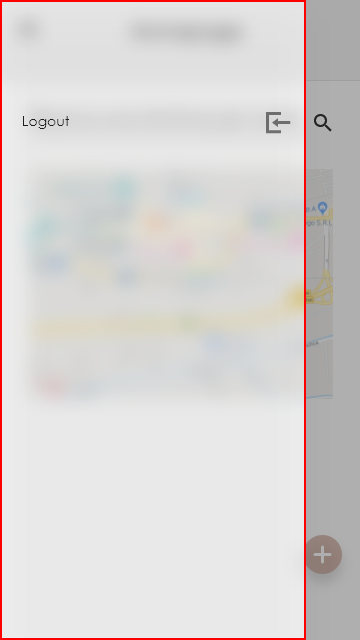
\includegraphics[scale=0.4]{Figures/DrawerUtenteL.png}
    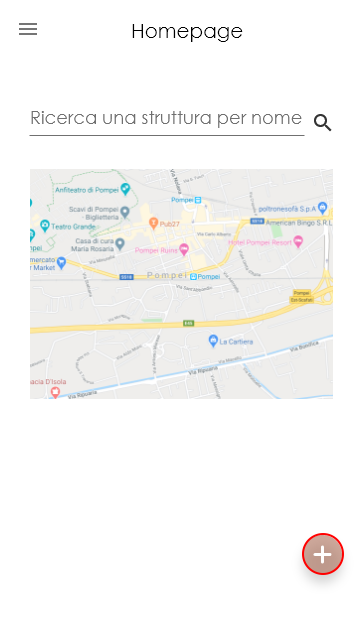
\includegraphics[scale=0.4]{Figures/HomePageUtenteL.png} 
\end{figure}

%%%%% ===============================================================================


% ===========================================================================
%
%		FEDERICO II THESIS TEMPLATE - ENGLISH
%  					* an example of Chapter 1: information about the discussion of the thesis
%	 
% 		AUTHOR:  		Antonio Esposito (antonio.esposito103@studenti.unina.it)
%		LAST UPDATED:	2017/06/20
%
% ===========================================================================

\chapter{Modello di Dominio}

%%%%% ===============================================================================
%\section{Classi, oggetti e relazioni di analisi}
%Qua vanno messi i class diagram
%%%%% ===============================================================================
\section{Diagrammi di sequenza di analisi}
Si riportano di seguito i diagrammi di sequenza di analisi dei casi d'uso.
\includepdf[pages={1-6}]{SequenceAnalisi/diagrammi.pdf}

\pagebreak
%%%%% ===============================================================================
\section{Diagrammi di stato di attività}
Sono riportati di seguito i diagrammi di stato di alcuni casi d'uso.
\begin{figure}[h!]
    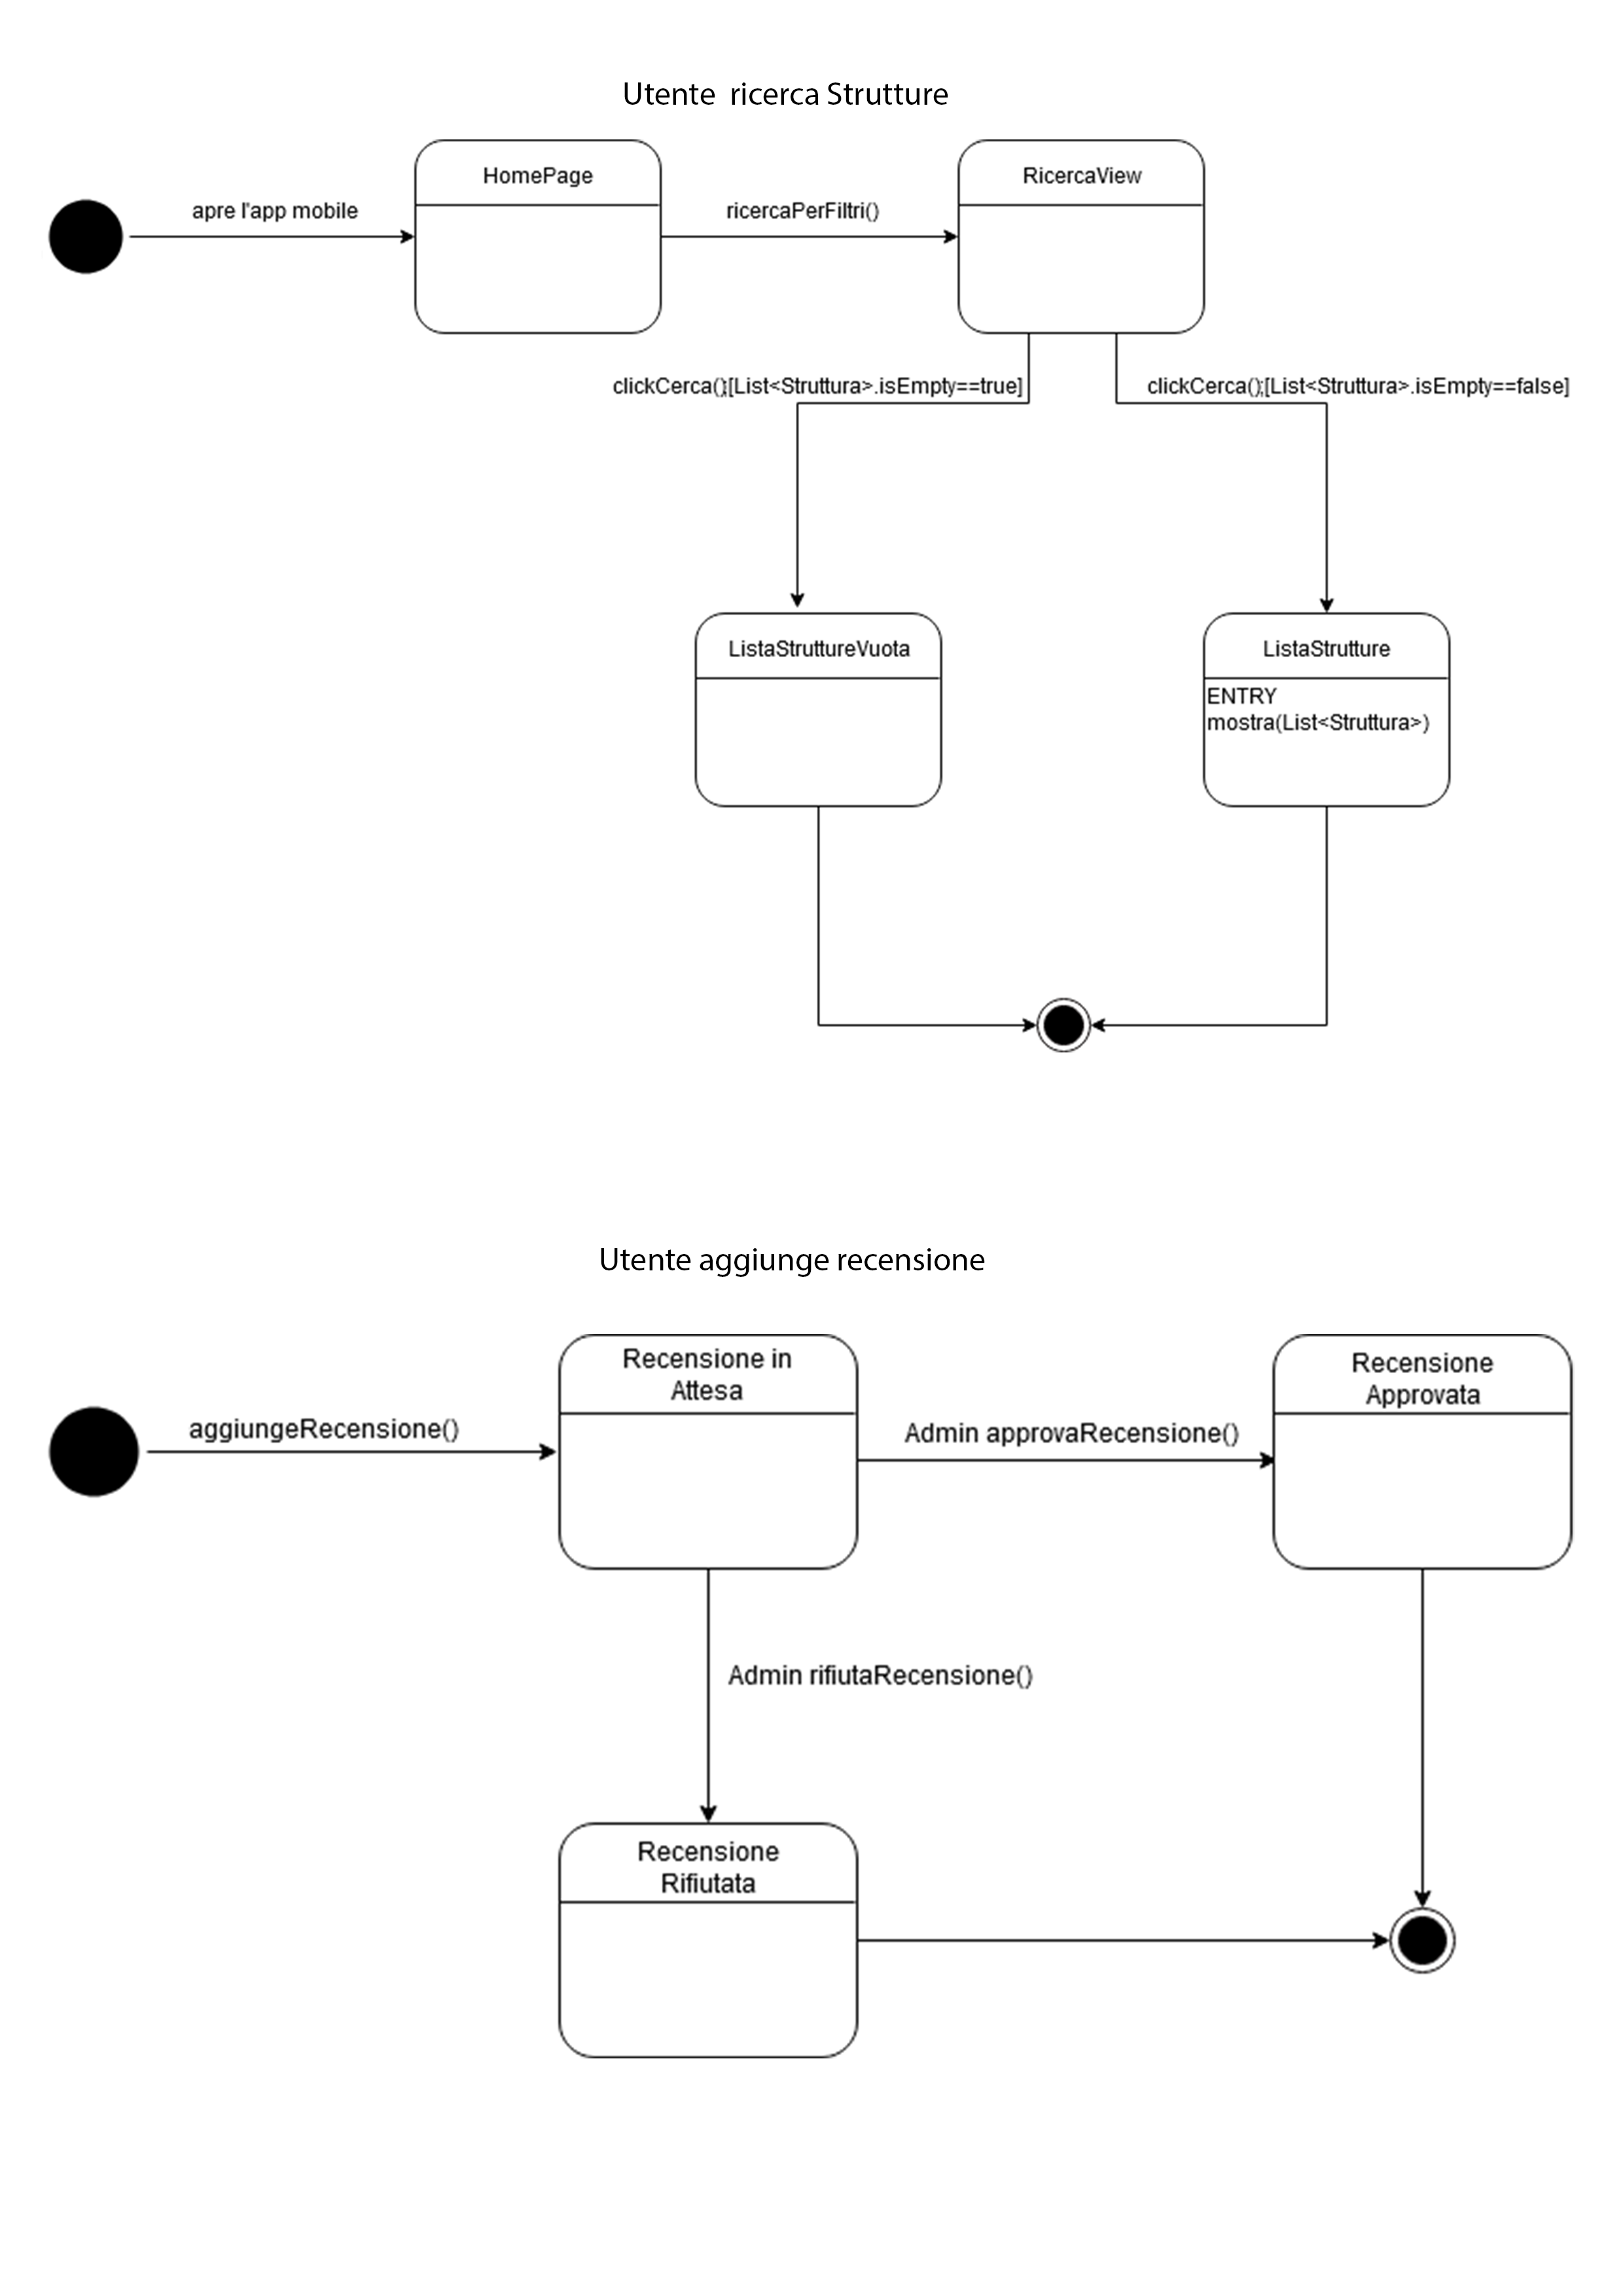
\includegraphics[width=\textwidth]{SequenceAnalisi/7.png}
\end{figure}
\begin{figure}[h!]
    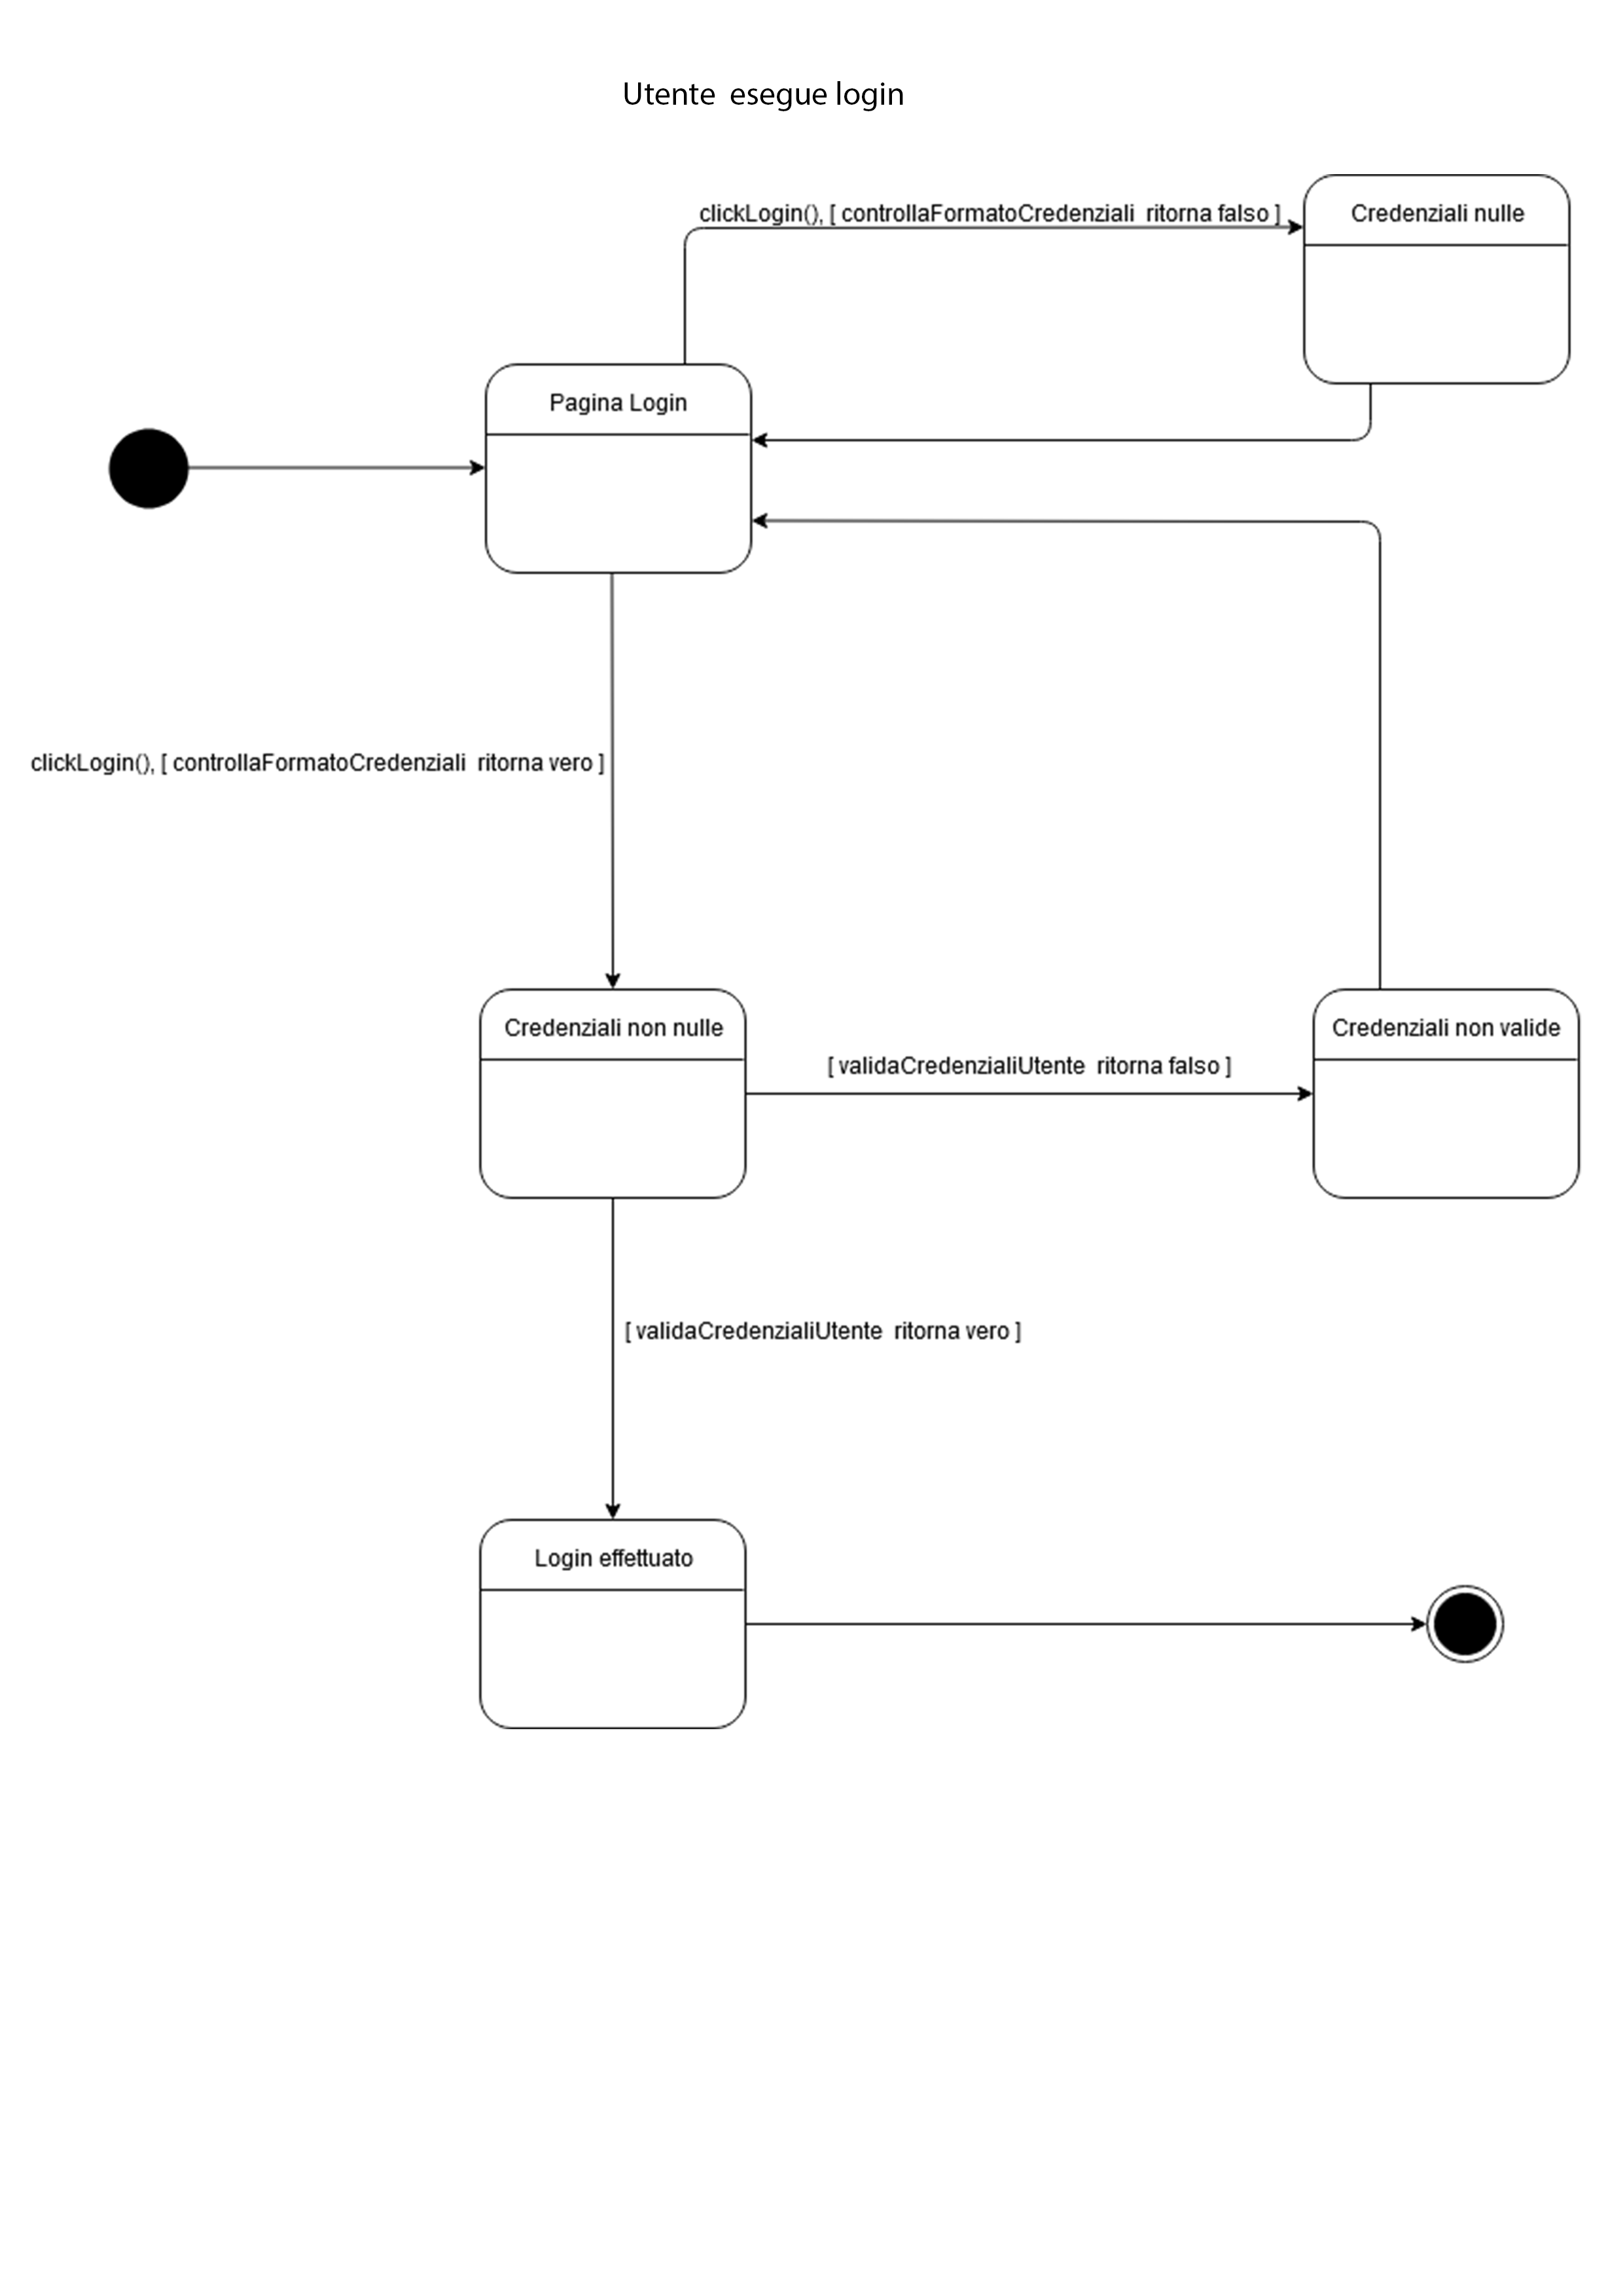
\includegraphics[width=\textwidth]{SequenceAnalisi/8.png}
\end{figure}
\pagebreak
%%%%% ===============================================================================
\section{Diagrammi di attività}
Sono riportati di seguito i diagrammi di attività di alcuni casi d'uso.
\begin{figure}[h!]
    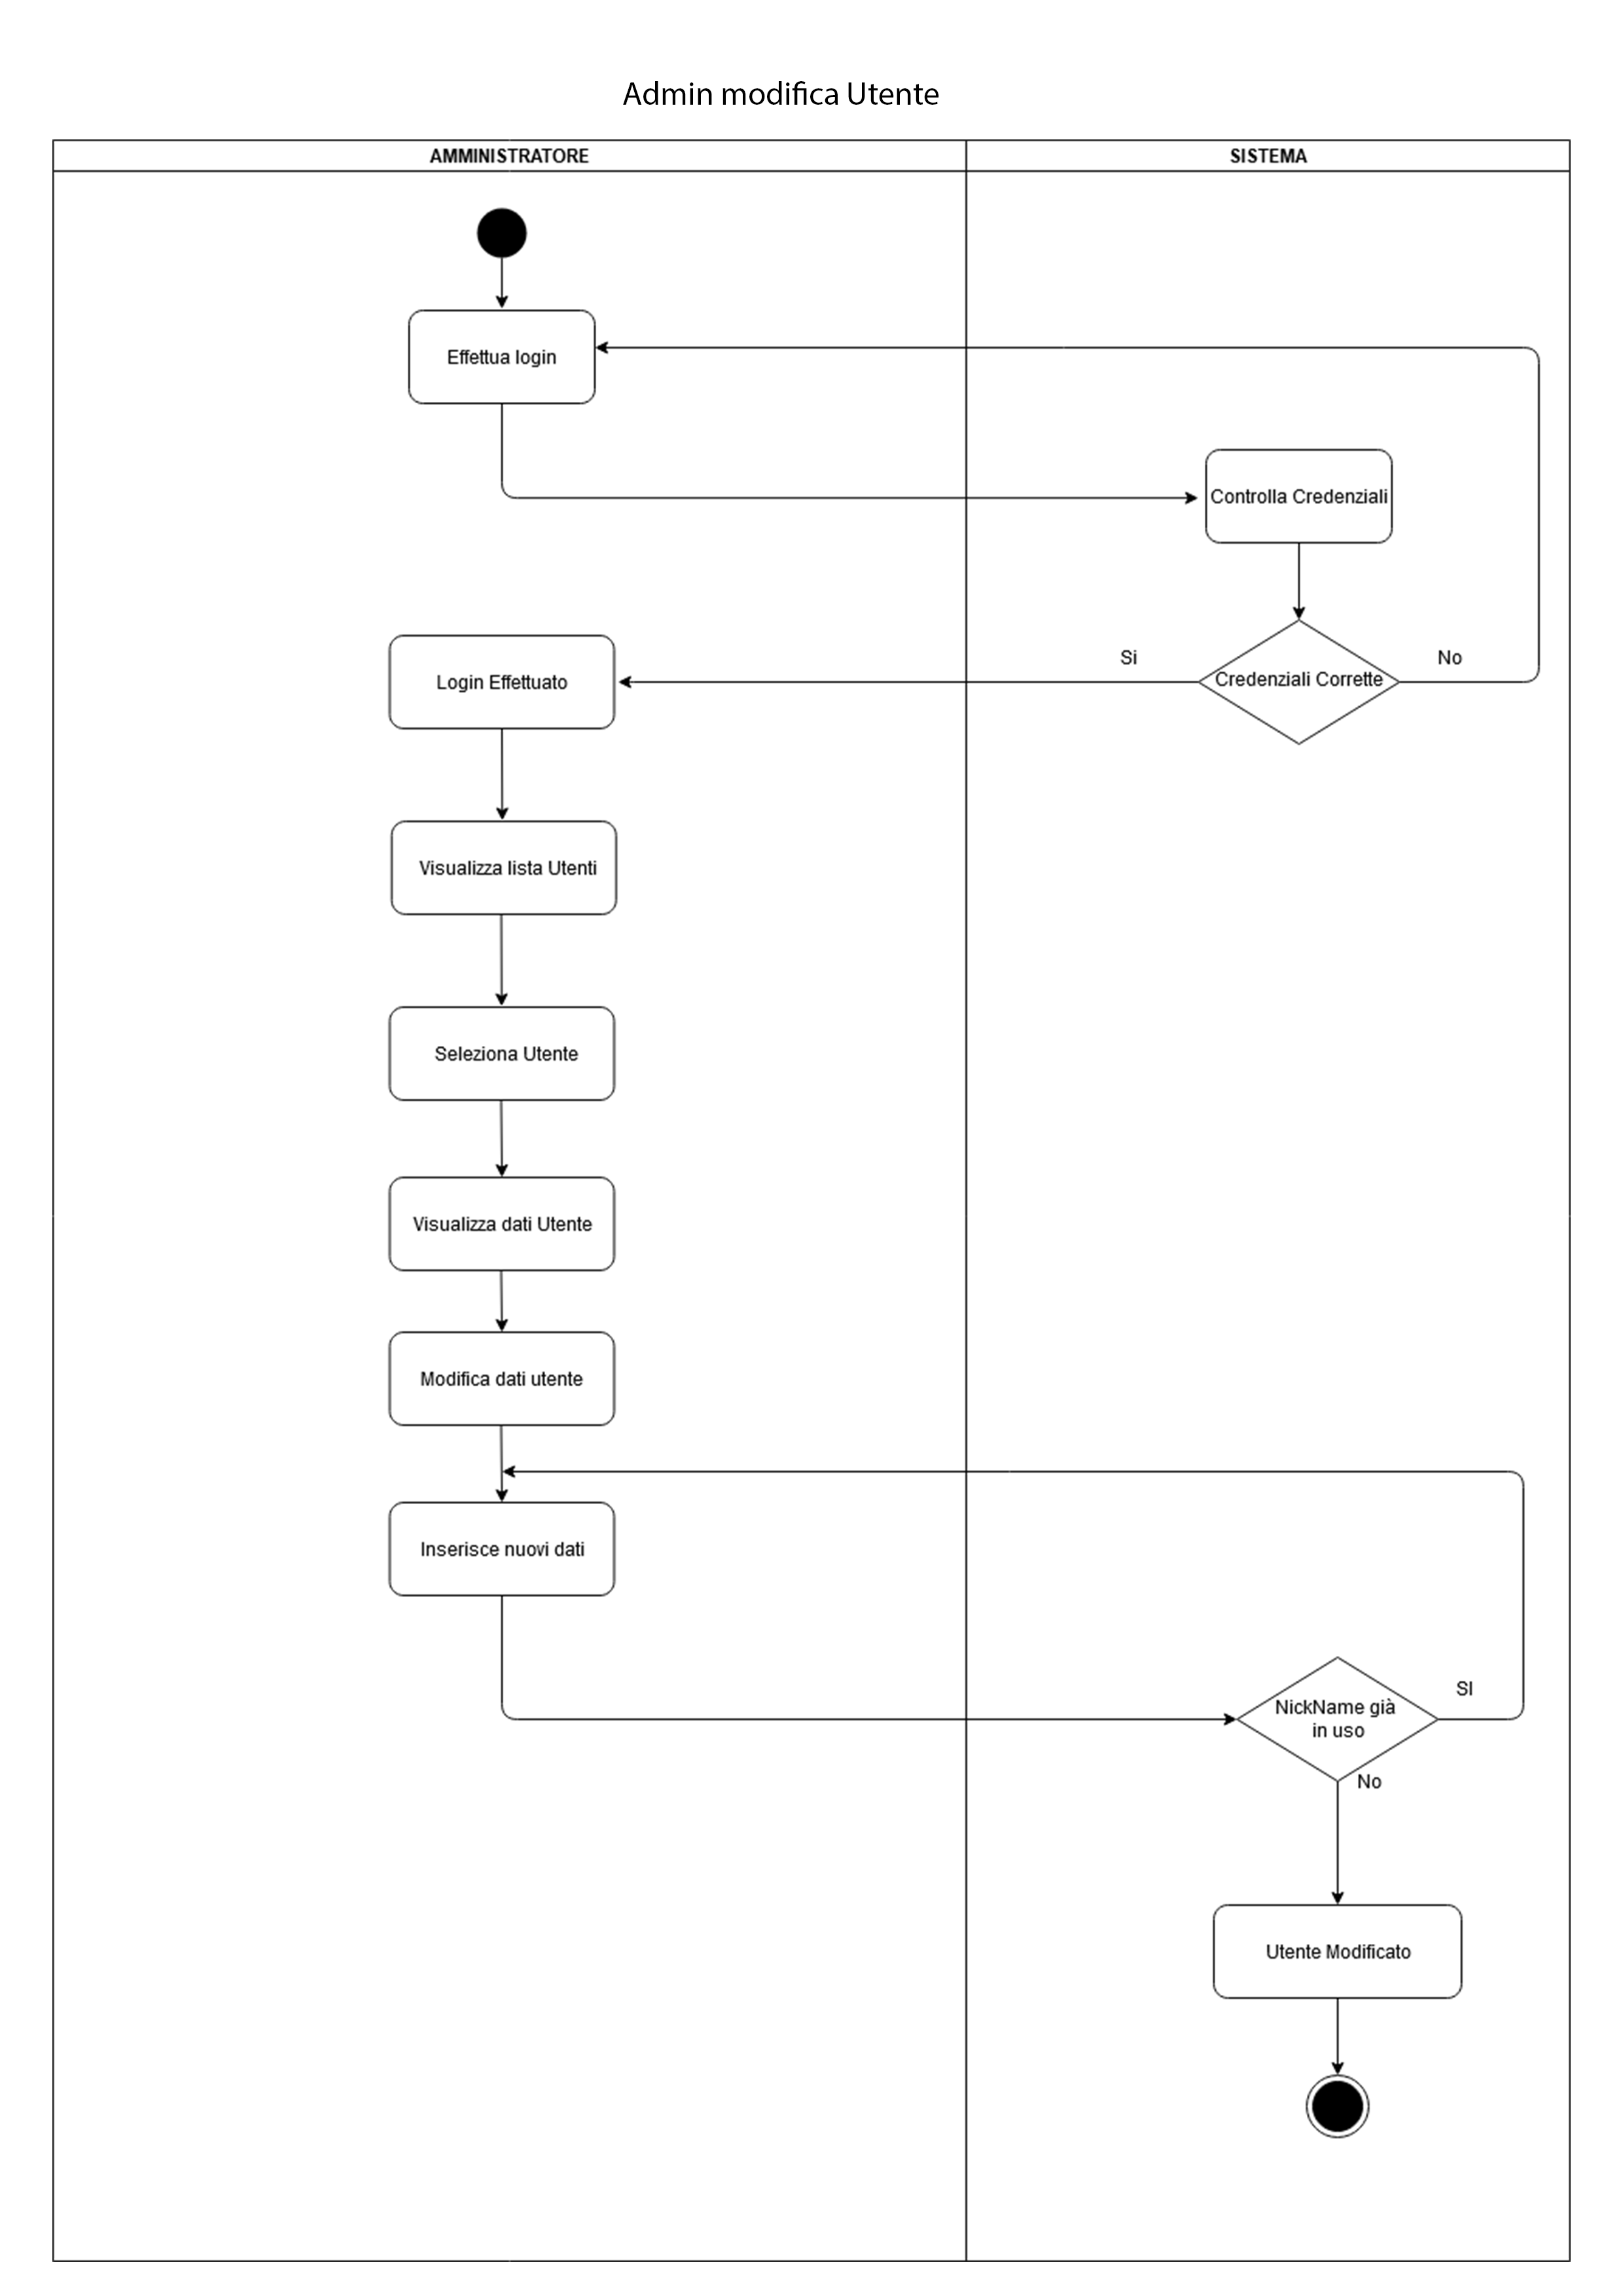
\includegraphics[width=\textwidth]{SequenceAnalisi/9.png}
\end{figure}
\begin{figure}[h!]
    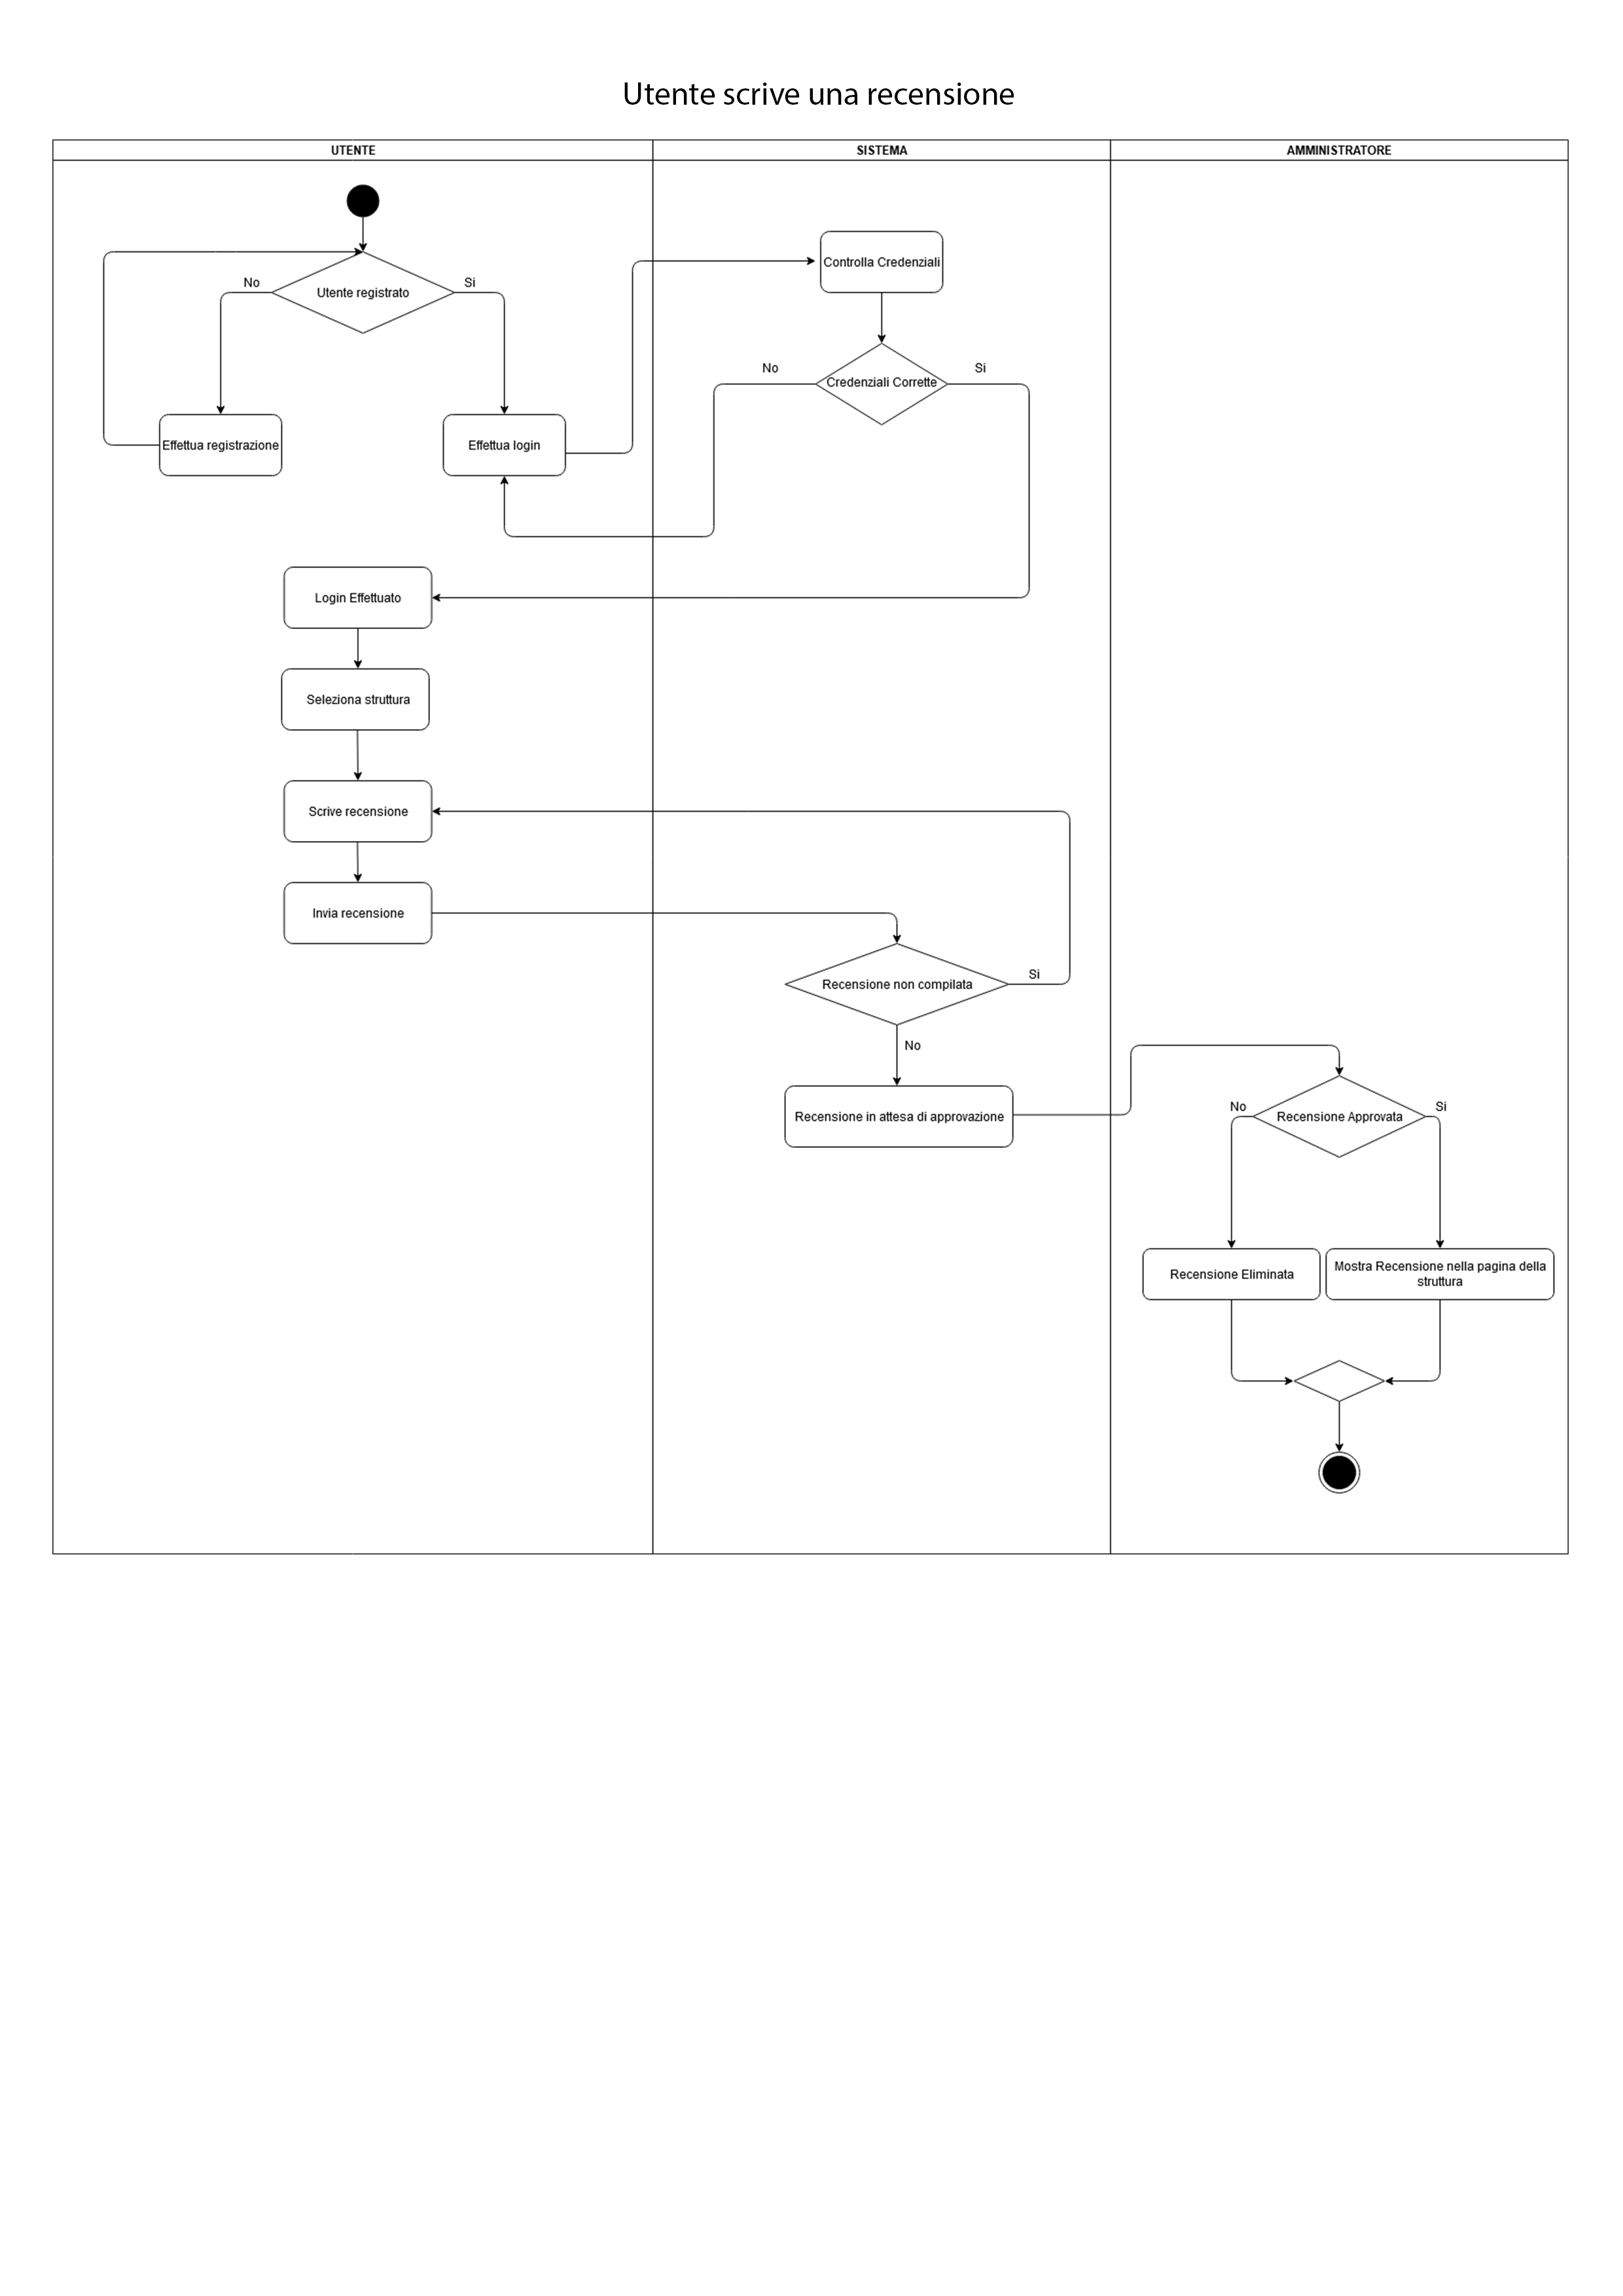
\includegraphics[width=\textwidth]{SequenceAnalisi/10.png}
\end{figure}
\begin{figure}[h!]
    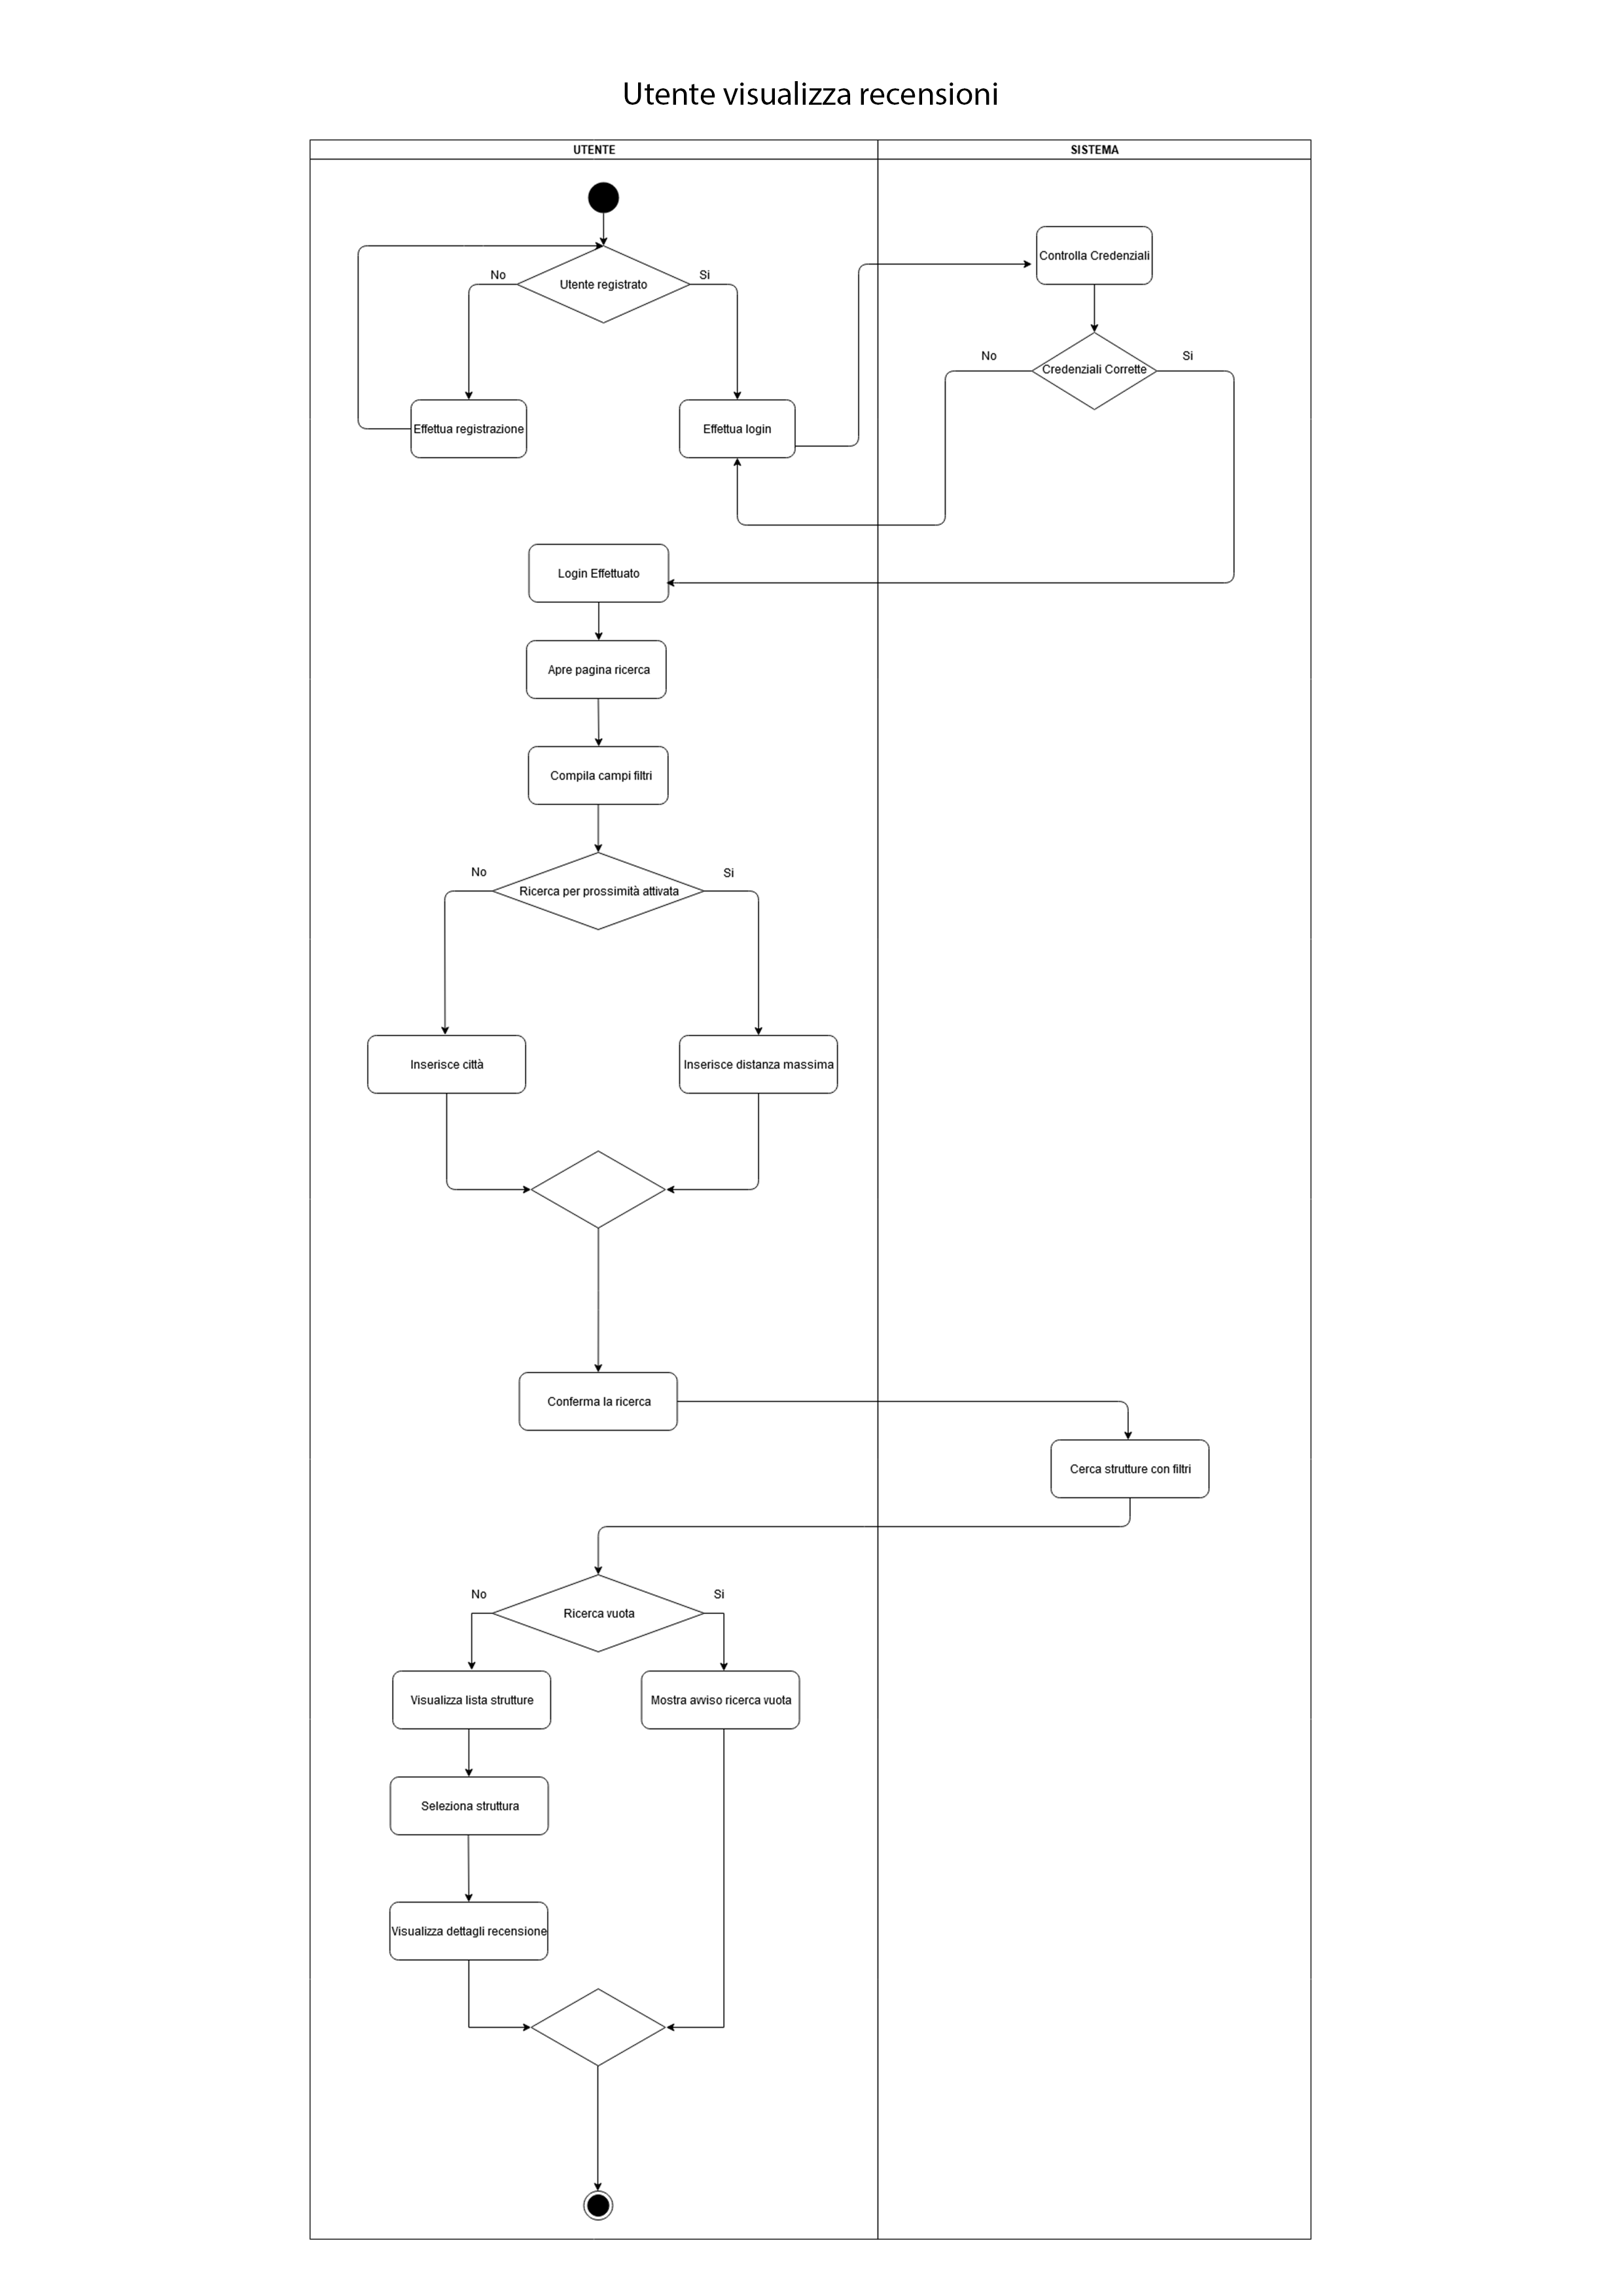
\includegraphics[width=\textwidth]{SequenceAnalisi/11.png}
\end{figure}

%%%%% ===============================================================================

% ===========================================================================
%
%		FEDERICO II THESIS TEMPLATE - ENGLISH
%  					* an example of Chapter 1: information about the discussion of the thesis
%	 
% 		AUTHOR:  		Antonio Esposito (antonio.esposito103@studenti.unina.it)
%		LAST UPDATED:	2017/06/20
%
% ===========================================================================

\chapter{Impegno risorse e pianificazione dell'attività}

This chapter contains useful information for the preparation and the presentation of the master degree thesis for students of Electronic Engineering (M61), at the University of Study of Naples Federico II.

The final test for the Master Degree course in Electronic Engineering consists in the preparation and discussion of a thesis, written with the help of a supervisor (eventually with one or two co-supervisors). This work is the final result of the student career and it testifies his/her ability in exploring in deep the topics encountered during the degree course.

%%%%% ===============================================================================
\section{Diagrammi di Grant}

\part{Documento di Design del sistema}
% ===========================================================================
%
%		FEDERICO II THESIS TEMPLATE - ENGLISH
%  					* an example of Chapter 2: mathematical text
%	 
% 		AUTHOR:  		Antonio Esposito (antonio.esposito103@studenti.unina.it)
%		LAST UPDATED:	2017/06/20
%
% ===========================================================================

\chapter{Design}
\section{Descrizione del dominio}
In seguito ad un'analisi dei requisiti del sistema si è resa evidente l'esistenza di alcune entità
principali:
\begin{itemize}
    \item gli \textit{Utenti} che possono registrarsi, visualizzare delle \textit{Strutture}
    e scrivere delle recensioni
    \item degli \textit{Amministratori} i quali possono gestire i dati dei visitatori e le loro recensioni
\end{itemize}
%%%%% ===============================================================================
\section{Analisi dell'architettura}
Il sistema si basa principalmente su due pattern architetturali: Client-Server e Model-View-Controller.\\
Il sistema infatti è composto da diversi client che tramite internet interagiscono con un Server remoto.
\begin{center}
    \begin{figure}[H]
        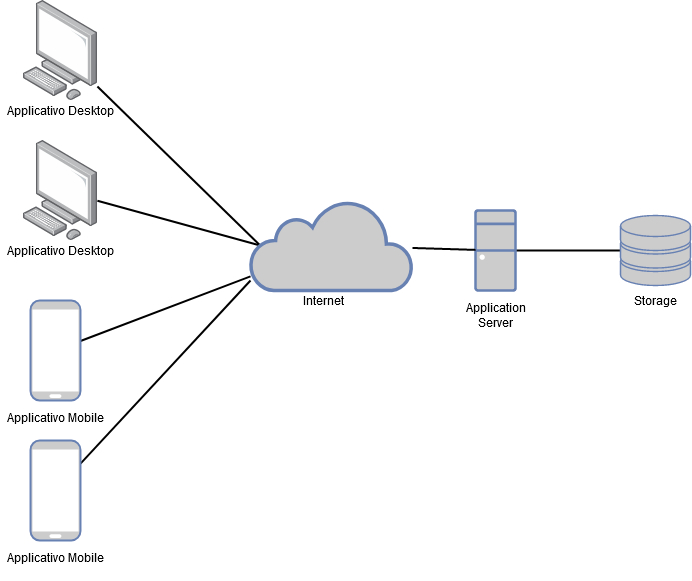
\includegraphics[width=\textwidth]{Figures/Architettura client server.png}
        \caption{Architettura client server}
    \end{figure}
\end{center}
\subsection{Model-View-Presenter}
Per quanto riguarda l'architettura interna dei client si è deciso di utilizzare il modello Model-View-Presenter (variante Passive View)
favorendo la separazione dei componenti software del sistema e separandone le responsabilità.
In questo modo si riesce ad ottenere alta coesione e basso accoppiamento, ottenendo una buona manutenibilà.\\
A favore di ciò il progetto è diviso in tre sottocartelle principali: Model, View e Presenter.\\
\\
Il modello MVP è un'evoluzione del modello Model View Controller ed è usato principalmente per creare user interfaces 
ed in particolare nella variante Passive View:
la componente \textbf{View} è completamente passiva e statica deputata soltanto alla visualizzazione dei dati.\\
la componente \textbf{Model} ha la responsabilità di fornire i metodi per accedere
ai dati utili all'applicazione, ha conoscenza del dominio applicativo ed è indipendente
dagli altri sottosistemi.\\
la componente \textbf{Presenter} fa da "middle man" tra la View ed il Model e si occupa di prendere i dati dal model, 
fornirli alla view e gestire gli input dell'utente
\begin{center}
    \begin{figure}[H]
        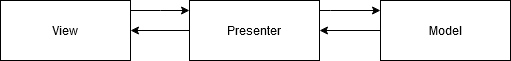
\includegraphics[width=\textwidth]{Figures/MVP client.png}
        \caption{Architettura Model-View-Controller}
    \end{figure}
\end{center}
\section{Diagramma delle classi di design}
\phantomsection
\addcontentsline{toc}{subsection}{Applicativo Desktop}
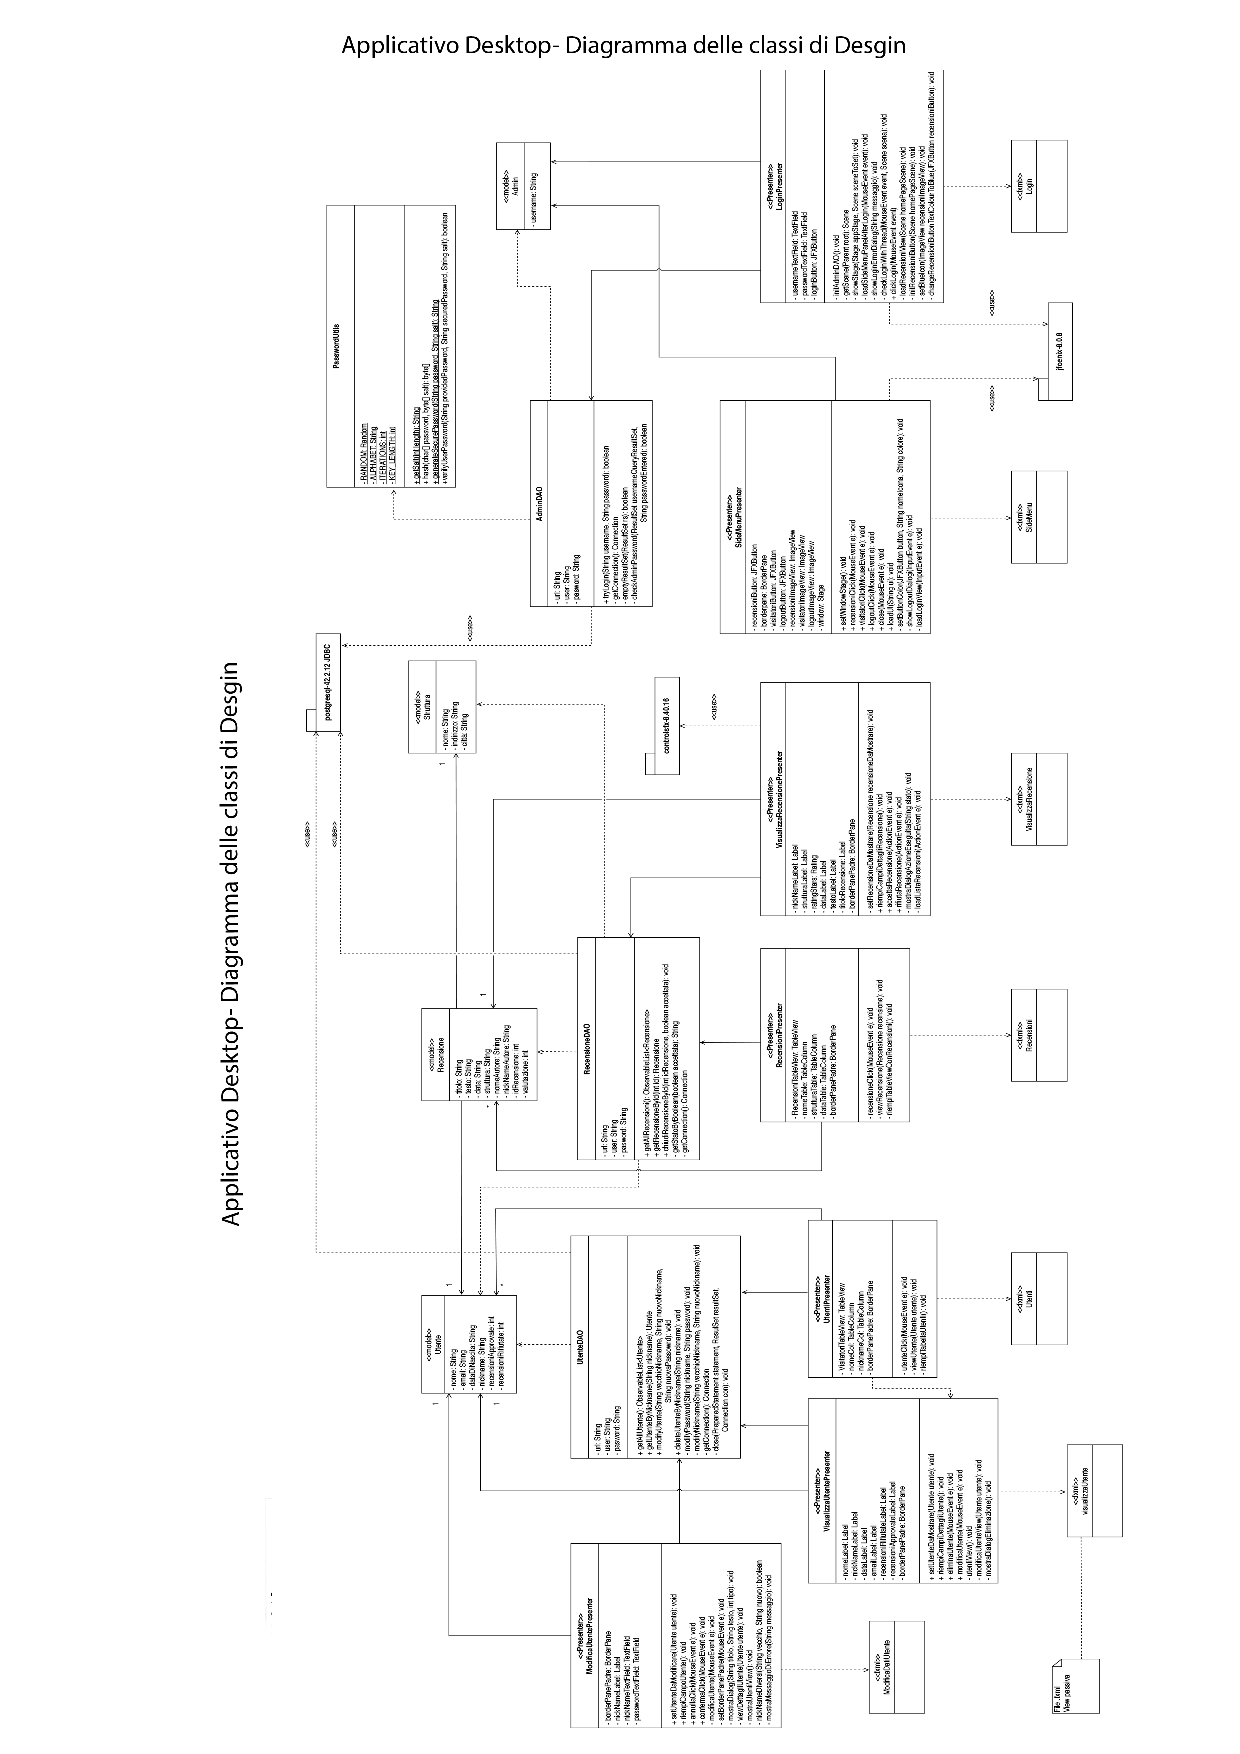
\includepdf{Class Diagram/Design/Desktop.pdf}
\pagebreak
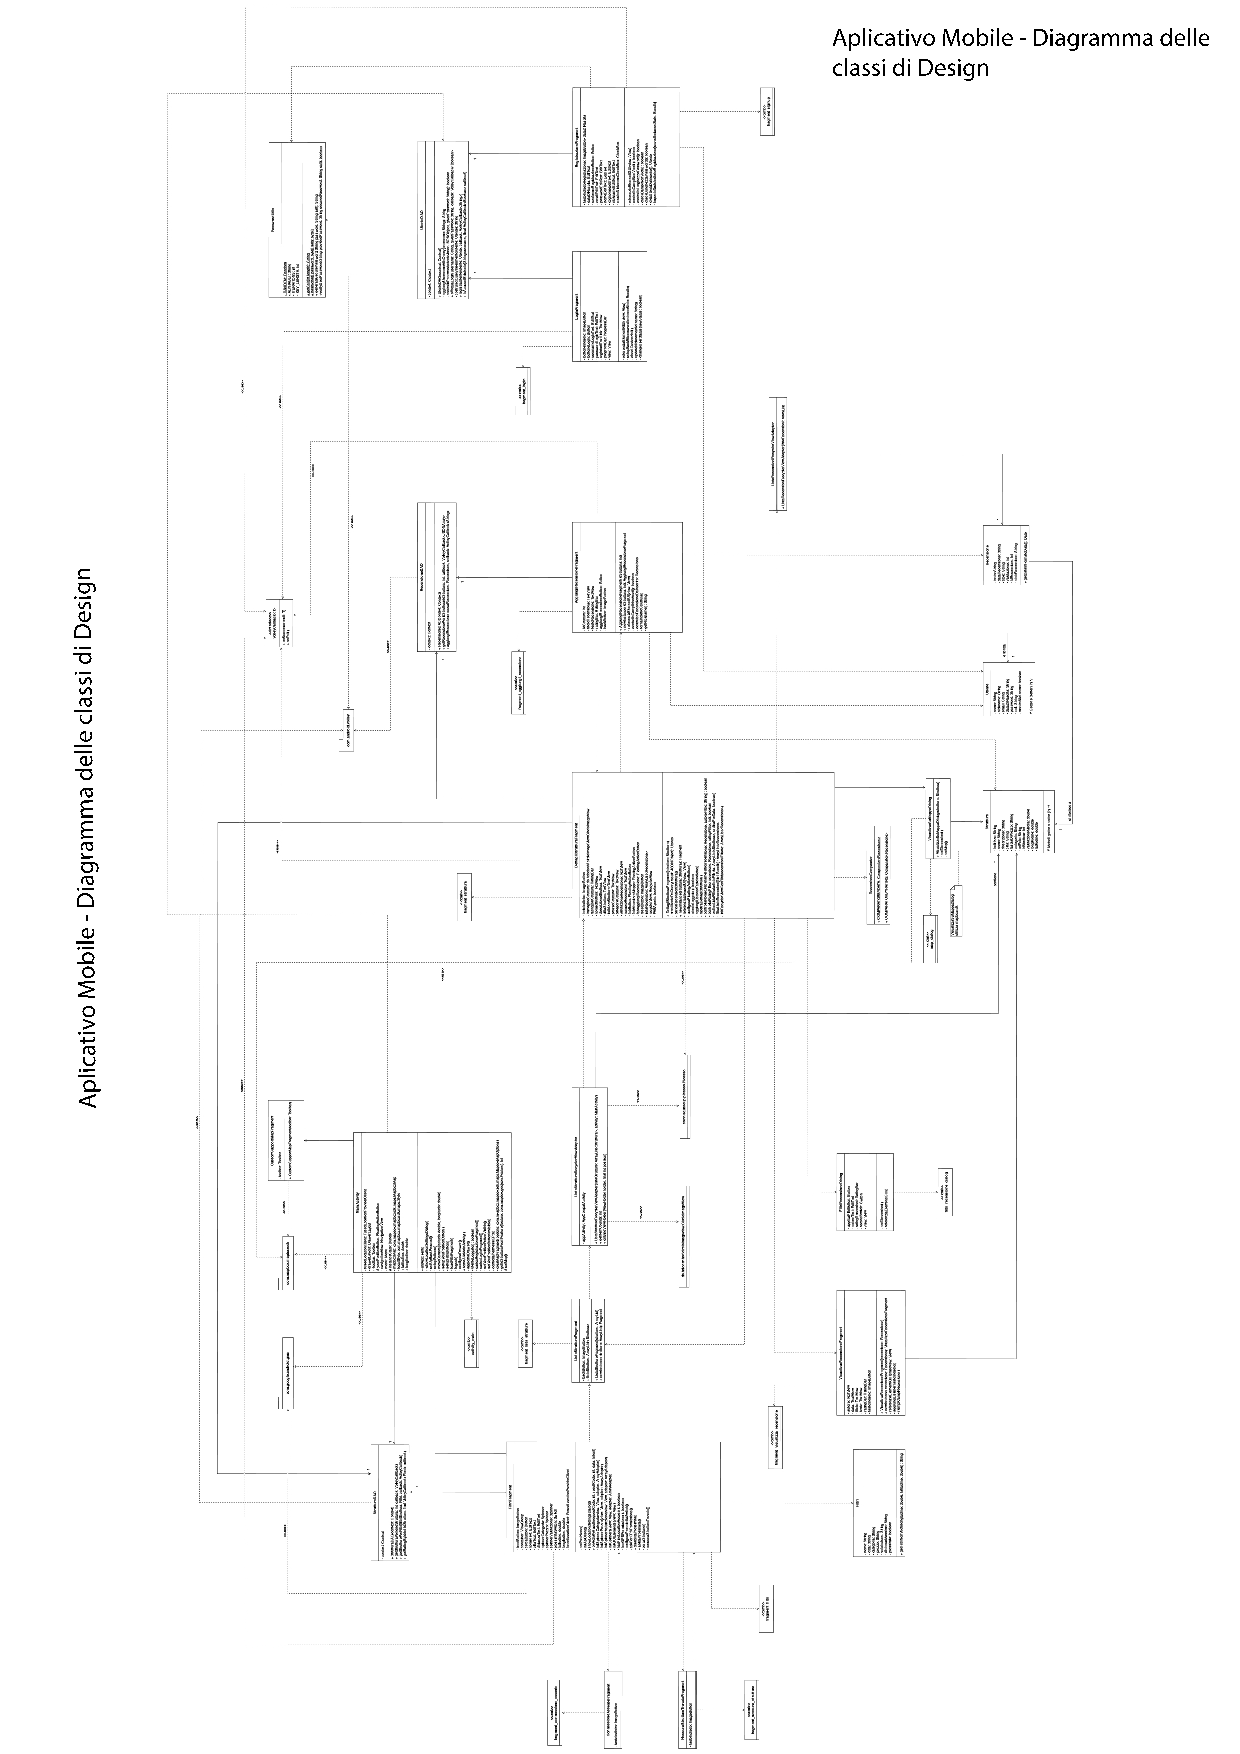
\includepdf{Class Diagram/Design/Mobile.pdf}
\addcontentsline{toc}{subsection}{Applicativo Mobile}
%------------------------------------
\section{CRC  Cards}
Di seguitop sono riportate tutte le Class Responsability Collaboration(CRC) del prodotto.

\subsection{Entità}
    
%Intestazione tabella%
\setcounter{table}{0}
\begin{table}[H]
    \centering
    %\caption{AdminDAO} 
    \begin{tabular}{||   l  ||  c   ||}
        \rowcolor{Gray}
        \hline
        Nome Classe & Recensione\\
        \hline
        Superclasse  &  - \\
        \hline
        Sottoclassi & - \\
        \hline
        \hline
         Responsabilità & Collaboratore \\
         \hline
          Rappresentare l'entità Recensione & Utente, Struttura \\
         \hline
    \end{tabular}
    %Continua alla pagina seguente
\end{table}

    
       

    
%Intestazione tabella%
\setcounter{table}{0}
\begin{table}[H]
    \centering
    %\caption{AdminDAO} 
    \begin{tabular}{||   l  ||  c   ||}
        \hline
        Nome Classe & Struttura\\
        \hline
        Superclassi  &  - \\
        \hline
        Sottoclassi & - \\
        \hline
        \hline
         Responsabilità & Collaboratore \\
         \hline
          Rappresentare l'entità Struttura & - \\
         \hline
    \end{tabular}
    %Continua alla pagina seguente
\end{table}

    
       
 
    
%Intestazione tabella%
\setcounter{table}{0}
\begin{table}[H]
    \centering
    %\caption{AdminDAO} 
    \begin{tabular}{||   l  ||  c   ||}
        \hline
        Nome Classe & RecensioneDAO\\
        \hline
        Superclassi  &  - \\
        \hline
        Sottoclassi & - \\
        \hline
         Responsabilità & Collaboratore \\
         \hline
          Effettuare le operazioni CRUD per l'entità Recensione & - \\
         \hline
    \end{tabular}
    %Continua alla pagina seguente
\end{table}

    
%Intestazione tabella%
\setcounter{table}{0}
\begin{table}[H]
    \centering
    %\caption{AdminDAO} 
    \begin{tabular}{||   l  ||  c   ||}
        \hline
        Nome Classe & AdminDAO\\
        \hline
        Superclassi  &  - \\
        \hline
        Sottoclassi & - \\
        \hline
         Responsabilità & Collaboratore \\
         \hline
          Effettuare le operazioni CRUD per l'entità Admin & - \\
         \hline
    \end{tabular}
    %Continua alla pagina seguente
\end{table}

    
       

    
%Intestazione tabella%
\setcounter{table}{0}
\begin{table}[H]
    \centering
    %\caption{AdminDAO} 
    \begin{tabular}{||   l  ||  c   ||}
        \hline
        Nome Classe & RecensioneDAO\\
        \hline
        Superclassi  &  - \\
        \hline
        Sottoclassi & - \\
        \hline
         Responsabilità & Collaboratore \\
         \hline
          Effettuare le operazioni CRUD per l'entità Recensione & - \\
         \hline
    \end{tabular}
    %Continua alla pagina seguente
\end{table}

\subsection{Applicativo Desktop} 
    
%Intestazione tabella%
\setcounter{table}{0}
\begin{table}[H]
    \centering
    \begin{tabular}{||   l  ||  c   ||}
        \rowcolor{Gray}
        \hline
        Nome Classe & AdminDAO\\
        \hline
        Superclasse  &  - \\
        \hline
        Sottoclassi & - \\
        \hline
        \hline
         Responsabilità & Collaboratore \\
         \hline
          Effettuare le operazioni CRUD per l'entità Admin & - \\
         \hline
    \end{tabular}
    
    %Continua alla pagina seguente
\end{table}

    
       

    
%Intestazione tabella%
\setcounter{table}{0}
\begin{table}[H]
    \centering
    %\caption{AdminDAO}
    \begin{tabularx}{\textwidth}{||   X  ||  c   ||}
        \rowcolor{Gray}
        \hline
        \textbf{Nome Classe} & UtenteDAO \\
        \hline
        \textbf{Superclasse}  &  - \\
        \hline
        \textbf{Sottoclassi} & - \\
        \hline
        \hline
         \textbf{Responsabilità} & \textbf{Collaboratore} \\
         \hline
          Effettuare le operazioni \gls{CRUD} per l'entità Utente tramite richiesta GET HTTP al web service & - \\
         \hline
    \end{tabularx}
    %Continua alla pagina seguente
\end{table}

    
%Intestazione tabella%
\setcounter{table}{0}
\begin{table}[H]
    \centering
    %\caption{AdminDAO} 
    \begin{tabular}{||   l  ||  c   ||}
        \rowcolor{Gray}
        \hline
        Nome Classe & RecensioneDAO\\
        \hline
        Superclasse  &  - \\
        \hline
        Sottoclassi & - \\
        \hline
        \hline
         Responsabilità & Collaboratore \\
         \hline
          Effettuare le operazioni CRUD per l'entità Recensione & - \\
         \hline
    \end{tabular}
    %Continua alla pagina seguente
\end{table}

    
       

    
%Intestazione tabella%
\setcounter{table}{0}
\begin{table}[H]
    \centering
    %\caption{AdminDAO} 
    \begin{tabular}{||   l  ||  c   ||}
        \rowcolor{Gray}
        \hline
        \textbf{Nome Classe} & LoginPresenter\\
        \hline
        \textbf{Superclasse}  &  - \\
        \hline
        \textbf{Sottoclassi} & - \\
        \hline
        \hline
         \textbf{Responsabilità} & \textbf{Collaboratore} \\
         \hline
          Gestire l'interazione per il login & AdminDAO, Admin \\
         \hline
    \end{tabular}
    %Continua alla pagina seguente
\end{table}


       

    
%Intestazione tabella%
\setcounter{table}{0}
\begin{table}[H]
    \centering
    %\caption{AdminDAO} 
    \begin{tabular}{||   l  ||  c   ||}
        \hline
        \rowcolor{Gray}
        \textbf{Nome Classe} & SideMenuPresenter\\
        \hline
        \textbf{Superclasse}  &  - \\
        \hline
        \textbf{Sottoclassi} & - \\
        \hline
        \hline
         \textbf{Responsabilità} & \textbf{Collaboratore} \\
         \hline
          Gestire l'interazione con la SideBar & Admin \\
         \hline
    \end{tabular}
    %Continua alla pagina seguente
\end{table}

    
       

    
%Intestazione tabella%
\setcounter{table}{0}
\begin{table}[H]
    \centering
    %\caption{AdminDAO} 
    \begin{tabularx}{\textwidth}{||  X  ||  c   ||}
        \rowcolor{Gray}
        \rowcolor{Gray}
        \hline
        \textbf{Nome Classe} & ModificaUtentePresenter\\
        \hline
        \textbf{Superclasse}  &  - \\
        \hline
        \textbf{Sottoclassi} & - \\
        \hline
        \hline
         \textbf{Responsabilità} & \textbf{Collaboratore} \\
         \hline
          Gestire l'interazione per la modifica\newline dei dati di accesso di un utente & Utente, UtenteDAO \\
         \hline
    \end{tabularx}
    %Continua alla pagina seguente
\end{table}

    
       

    
%Intestazione tabella%
\setcounter{table}{0}
\begin{table}[H]
    \centering
    %\caption{AdminDAO} 
    \begin{tabular}{||   l  ||  c   ||}
        \rowcolor{Gray}
        \hline
        \textbf{Nome Classe} & RecensioniPresenter\\
        \hline
        \textbf{Superclasse}  &  - \\
        \hline
        \textbf{Sottoclassi} & - \\
        \hline
        \hline
         \textbf{Responsabilità} & \textbf{Collaboratore} \\
         \hline
          Riempire la tabella con le recensioni in attesa di approvazione & RecensioneDAO \\
         \hline
    \end{tabular}
    %Continua alla pagina seguente
\end{table}

    
       

    
%Intestazione tabella%
\setcounter{table}{0}
\begin{table}[H]
    \centering
    %\caption{AdminDAO} 
    \begin{tabular}{||   l  ||  c   ||}
        \hline
        \rowcolor{Gray}
        \textbf{Nome Classe} & UtentiPresenter\\
        \hline
        \textbf{Superclasse}  &  - \\
        \hline
        \textbf{Sottoclassi} & - \\
        \hline
        \hline
         \textbf{Responsabilità} & \textbf{Collaboratore} \\
         \hline
         Riempire la tabella con gli utenti registrati alla piattaforma & UtenteDAO \\
         \hline
    \end{tabular}
    %Continua alla pagina seguente
\end{table}

    
       

    
%Intestazione tabella%
\setcounter{table}{0}
\begin{table}[H]
    \centering
    %\caption{AdminDAO} 
    \begin{tabular}{||   l  ||  c   ||}
        \hline
        \rowcolor{Gray}
        \textbf{Nome Classe} & VisualizzaRecensionePresenter\\
        \hline
        \textbf{Superclasse}  &  - \\
        \hline
        \textbf{Sottoclassi} & - \\
        \hline
        \hline
         \textbf{Responsabilità} & \textbf{Collaboratore} \\
         \hline
          Gestire l'interazione per la moderazione\newline di una recensione da parte di un admin & RecensioneDAO, Recensione \\
         \hline
    \end{tabular}
    %Continua alla pagina seguente
\end{table}

    
       

    
%Intestazione tabella%
\setcounter{table}{0}
\begin{table}[H]
    \centering
    %\caption{AdminDAO} 
    \begin{tabularx}{\textwidth}{||   X  ||  c   ||}
        \hline
        \rowcolor{Gray}
        \textbf{Nome Classe} & VisualizzaUtentePresenter\\
        \hline
        \textbf{Superclasse}  &  - \\
        \hline
        \textbf{Sottoclassi} & - \\
        \hline
        \hline
         \textbf{Responsabilità} & \textbf{Collaboratore} \\
         \hline
          Mostrare i dati completi di un utente & UtenteDAO, Utente \\
         \hline
          Permette l'eliminazione dell'utente mostrato& UtenteDAO, Utente \\
         \hline
    \end{tabularx}
    %Continua alla pagina seguente
\end{table}

    
       

    
%Intestazione tabella%
\setcounter{table}{0}
\begin{table}[H]
    \centering
    %\caption{AdminDAO} 
    \begin{tabularx}{\textwidth}{||   X  ||  c   ||}
        \rowcolor{Gray}
        \hline
        \textbf{Nome Classe} & PasswordUtils\\
        \hline
        \textbf{Superclasse}  &  - \\
        \hline
        \textbf{Sottoclassi} & - \\
        \hline
        \hline
         \textbf{Responsabilità} & \textbf{Collaboratore} \\
         \hline
          Fornire funzionalità per il sistema di cifratura\newline delle password tramite sale (?)  & - \\
         \hline
    \end{tabularx}
    %Continua alla pagina seguente
\end{table}

    
       

    
%Intestazione tabella%
\setcounter{table}{0}
\begin{table}[H]
    \centering
    %\caption{AdminDAO} 
    \begin{tabular}{||   l  ||  c   ||}
        \rowcolor{Gray}
        \hline
        Nome Classe & AdminDAO\\
        \hline
        Superclasse  &  - \\
        \hline
        Sottoclassi & - \\
        \hline
         Responsabilità & Collaboratore \\
         \hline
          Effettuare le operazioni CRUD per l'entità Admin & - \\
         \hline
    \end{tabular}
    %Continua alla pagina seguente
\end{table}

    
       

    \pagebreak
\subsection{Applicativo Mobile}
    
%Intestazione tabella%
\setcounter{table}{0}
\begin{table}[H]
    \centering
    %\caption{AdminDAO}
    \begin{tabularx}{\textwidth}{||   X  ||  c   ||}
        \rowcolor{Gray}
        \hline
        \textbf{Nome Classe} & UtenteDAO \\
        \hline
        \textbf{Superclasse}  &  - \\
        \hline
        \textbf{Sottoclassi} & - \\
        \hline
        \hline
         \textbf{Responsabilità} & \textbf{Collaboratore} \\
         \hline
          Effettuare le operazioni \gls{CRUD} per l'entità Utente tramite richiesta GET HTTP al web service & - \\
         \hline
    \end{tabularx}
    %Continua alla pagina seguente
\end{table}

    
%Intestazione tabella%
\setcounter{table}{0}
\begin{table}[H]
    \centering
    %\caption{AdminDAO} 
    \begin{tabular}{||   l  ||  c   ||}
        \rowcolor{Gray}
        \hline
        Nome Classe & RecensioneDAO\\
        \hline
        Superclasse  &  - \\
        \hline
        Sottoclassi & - \\
        \hline
        \hline
         Responsabilità & Collaboratore \\
         \hline
          Effettuare le operazioni CRUD per l'entità Recensione & - \\
         \hline
    \end{tabular}
    %Continua alla pagina seguente
\end{table}

    
       

    
%Intestazione tabella%
\setcounter{table}{0}
\begin{table}[H]
    \centering
    %\caption{AdminDAO} 
    \begin{tabular}{||   l  ||  c   ||}
        \hline
        Nome Classe & RecensioneDAO\\
        \hline
        Superclassi  &  - \\
        \hline
        Sottoclassi & - \\
        \hline
         Responsabilità & Collaboratore \\
         \hline
          Effettuare le operazioni CRUD per l'entità Recensione & - \\
         \hline
    \end{tabular}
    %Continua alla pagina seguente
\end{table}

    
%Intestazione tabella%
\setcounter{table}{0}
\begin{table}[H]
    \centering
    %\caption{AdminDAO} 
    \begin{tabular}{||   l  ||  c   ||}
        \hline
        Nome Classe & RecensioneDAO\\
        \hline
        Superclassi  &  - \\
        \hline
        Sottoclassi & - \\
        \hline
         Responsabilità & Collaboratore \\
         \hline
          Effettuare le operazioni CRUD per l'entità Recensione & - \\
         \hline
    \end{tabular}
    %Continua alla pagina seguente
\end{table}

    
%Intestazione tabella%
\setcounter{table}{0}
\begin{table}[H]
    \centering
    %\caption{AdminDAO} 
    \begin{tabular}{||   l  ||  c   ||}
        \hline
        \rowcolor{Gray}
        \textbf{Nome Classe} & LoginFragment\\
        \hline
        Superclassi  &  - \\
        \hline
        \textbf{Sottoclassi} & - \\
        \hline
         \textbf{Responsabilità} & \textbf{Collaboratore} \\
         \hline
           Gestisce l'accesso, tramite credenziali, di un utente & UtenteDAO \\
         \hline
    \end{tabular}
    %Continua alla pagina seguente
\end{table}

    
%Intestazione tabella%
\setcounter{table}{0}
\begin{table}[H]
    \centering
    %\caption{AdminDAO} 
    \begin{tabular}{||   l  ||  c   ||}
        \hline
        Nome Classe & RecensioneDAO\\
        \hline
        Superclassi  &  - \\
        \hline
        Sottoclassi & - \\
        \hline
         Responsabilità & Collaboratore \\
         \hline
          Effettuare le operazioni CRUD per l'entità Recensione & - \\
         \hline
    \end{tabular}
    %Continua alla pagina seguente
\end{table}

    
%Intestazione tabella%
\setcounter{table}{0}
\begin{table}[H]
    \centering
    %\caption{AdminDAO} 
    \begin{tabular}{||   l  ||  c   ||}
        \hline
        Nome Classe & RecensioneDAO\\
        \hline
        Superclassi  &  - \\
        \hline
        Sottoclassi & - \\
        \hline
         Responsabilità & Collaboratore \\
         \hline
          Effettuare le operazioni CRUD per l'entità Recensione & - \\
         \hline
    \end{tabular}
    %Continua alla pagina seguente
\end{table}

    
%Intestazione tabella%
\setcounter{table}{0}
\begin{table}[H]
    \centering
    %\caption{AdminDAO} 
    \begin{tabular}{||   l  ||  c   ||}
        \hline
        Nome Classe & RecensioneDAO\\
        \hline
        Superclassi  &  - \\
        \hline
        Sottoclassi & - \\
        \hline
         Responsabilità & Collaboratore \\
         \hline
          Effettuare le operazioni CRUD per l'entità Recensione & - \\
         \hline
    \end{tabular}
    %Continua alla pagina seguente
\end{table}

    
%Intestazione tabella%
\setcounter{table}{0}
\begin{table}[H]
    \centering
    %\caption{AdminDAO} 
    \begin{tabular}{||   l  ||  c   ||}
        \hline
        Nome Classe & RecensioneDAO\\
        \hline
        Superclassi  &  - \\
        \hline
        Sottoclassi & - \\
        \hline
         Responsabilità & Collaboratore \\
         \hline
          Effettuare le operazioni CRUD per l'entità Recensione & - \\
         \hline
    \end{tabular}
    %Continua alla pagina seguente
\end{table}

    
%Intestazione tabella%
\setcounter{table}{0}
\begin{table}[H]
    \centering
    %\caption{AdminDAO} 
    \begin{tabularx}{\textwidth}{||   X  ||  c   ||}
        \hline
        \rowcolor{Gray}
        \textbf{Nome Classe} & DettagliStrutturaFragment\\
        \hline
        Superclassi  &  - \\
        \hline
        \textbf{Sottoclassi} & - \\
        \hline
        \hline
         \textbf{Responsabilità} & \textbf{Collaboratore} \\
         \hline
          Permette la visualizzazione dei dati di una struttura & Struttura, RecensioneDAO \\
         \hline
    \end{tabularx}
    %Continua alla pagina seguente
\end{table}

    
%Intestazione tabella%
\setcounter{table}{0}
\begin{table}[H]
    \centering
    %\caption{AdminDAO} 
    \begin{tabularx}{\textwidth}{||   X  ||  c   ||}
        \rowcolor{Gray}
        \hline
        \textbf{Nome Classe} & PasswordUtils\\
        \hline
        \textbf{Superclasse}  &  - \\
        \hline
        \textbf{Sottoclassi} & - \\
        \hline
        \hline
         \textbf{Responsabilità} & \textbf{Collaboratore} \\
         \hline
          Fornire funzionalità per il sistema di cifratura\newline delle password tramite sale (?)  & - \\
         \hline
    \end{tabularx}
    %Continua alla pagina seguente
\end{table}

    
       

    
%Intestazione tabella%
\setcounter{table}{0}
\begin{table}[H]
    \centering
    %\caption{AdminDAO} 
    \begin{tabularx}{\textwidth}{||   X  ||  c   ||}
        \hline
        \rowcolor{Gray}
        \textbf{Nome Classe} & NessunaStrutturaTrovata\\
        \hline
        Superclassi  &  - \\
        \hline
        \textbf{Sottoclassi} & - \\
        \hline
        \hline
         \textbf{Responsabilità} & \textbf{Collaboratore} \\
         \hline
           Mostra una schermata apposita nel caso in cui una ricerca
           non abbia nessun risultato da visualizzare & - \\
         \hline
    \end{tabularx}
    %Continua alla pagina seguente
\end{table}

    
%Intestazione tabella%
\setcounter{table}{0}
\begin{table}[H]
    \centering
    %\caption{AdminDAO} 
    \begin{tabularx}{\textwidth}{||   X  ||  c   ||}
        \hline
        \rowcolor{Gray}
        \textbf{Nome Classe} & VisualizzaRecensioneFragment\\
        \hline
        Superclassi  &  - \\
        \hline
        \textbf{Sottoclassi} & - \\
        \hline
         \textbf{Responsabilità} & \textbf{Collaboratore} \\
         \hline
          Permette la visualizzazione (con testo integrale) di una Recensione  & Recensione \\
         \hline
    \end{tabularx}
    %Continua alla pagina seguente
\end{table}

    
%Intestazione tabella%
\setcounter{table}{0}
\begin{table}[H]
    \centering
    %\caption{AdminDAO} 
    \begin{tabular}{||   l  ||  c   ||}
        \hline
        Nome Classe & RecensioneDAO\\
        \hline
        Superclassi  &  - \\
        \hline
        Sottoclassi & - \\
        \hline
         Responsabilità & Collaboratore \\
         \hline
          Effettuare le operazioni CRUD per l'entità Recensione & - \\
         \hline
    \end{tabular}
    %Continua alla pagina seguente
\end{table}
 
    
%Intestazione tabella%
\setcounter{table}{0}
\begin{table}[H]
    \centering
    %\caption{AdminDAO} 
    \begin{tabular}{||   l  ||  c   ||}
        \hline
        Nome Classe & RecensioneDAO\\
        \hline
        Superclassi  &  - \\
        \hline
        Sottoclassi & - \\
        \hline
         Responsabilità & Collaboratore \\
         \hline
          Effettuare le operazioni CRUD per l'entità Recensione & - \\
         \hline
    \end{tabular}
    %Continua alla pagina seguente
\end{table}

    
%Intestazione tabella%
\setcounter{table}{0}
\begin{table}[H]
    \centering
    %\caption{AdminDAO} 
    \begin{tabular}{||   l  ||  c   ||}
        \hline
        Nome Classe & RecensioneDAO\\
        \hline
        Superclassi  &  - \\
        \hline
        Sottoclassi & - \\
        \hline
         Responsabilità & Collaboratore \\
         \hline
          Effettuare le operazioni CRUD per l'entità Recensione & - \\
         \hline
    \end{tabular}
    %Continua alla pagina seguente
\end{table}
 
    
%Intestazione tabella%
\setcounter{table}{0}
\begin{table}[H]
    \centering
    %\caption{AdminDAO} 
    \begin{tabular}{||   l  ||  c   ||}
        \hline
        Nome Classe & RecensioneDAO\\
        \hline
        Superclassi  &  - \\
        \hline
        Sottoclassi & - \\
        \hline
         Responsabilità & Collaboratore \\
         \hline
          Effettuare le operazioni CRUD per l'entità Recensione & - \\
         \hline
    \end{tabular}
    %Continua alla pagina seguente
\end{table}

    
%Intestazione tabella%
\setcounter{table}{0}
\begin{table}[H]
    \centering
    %\caption{AdminDAO} 
    \begin{tabular}{||   l  ||  c   ||}
        \hline
        \rowcolor{Gray}
        \textbf{Nome Classe} & CustomSupportMapFragment\\
        \hline
        Superclassi  &  - \\
        \hline
        \textbf{Sottoclassi} & - \\
        \hline
         \textbf{Responsabilità} & \textbf{Collaboratore} \\
         \hline
          Gestisce la mappa visualizzata sull'homepage & - \\
         \hline
    \end{tabular}
    %Continua alla pagina seguente
\end{table}

%------------------------------------

\section{Diagrammi di sequenza di design}
\subsection{Desktop}
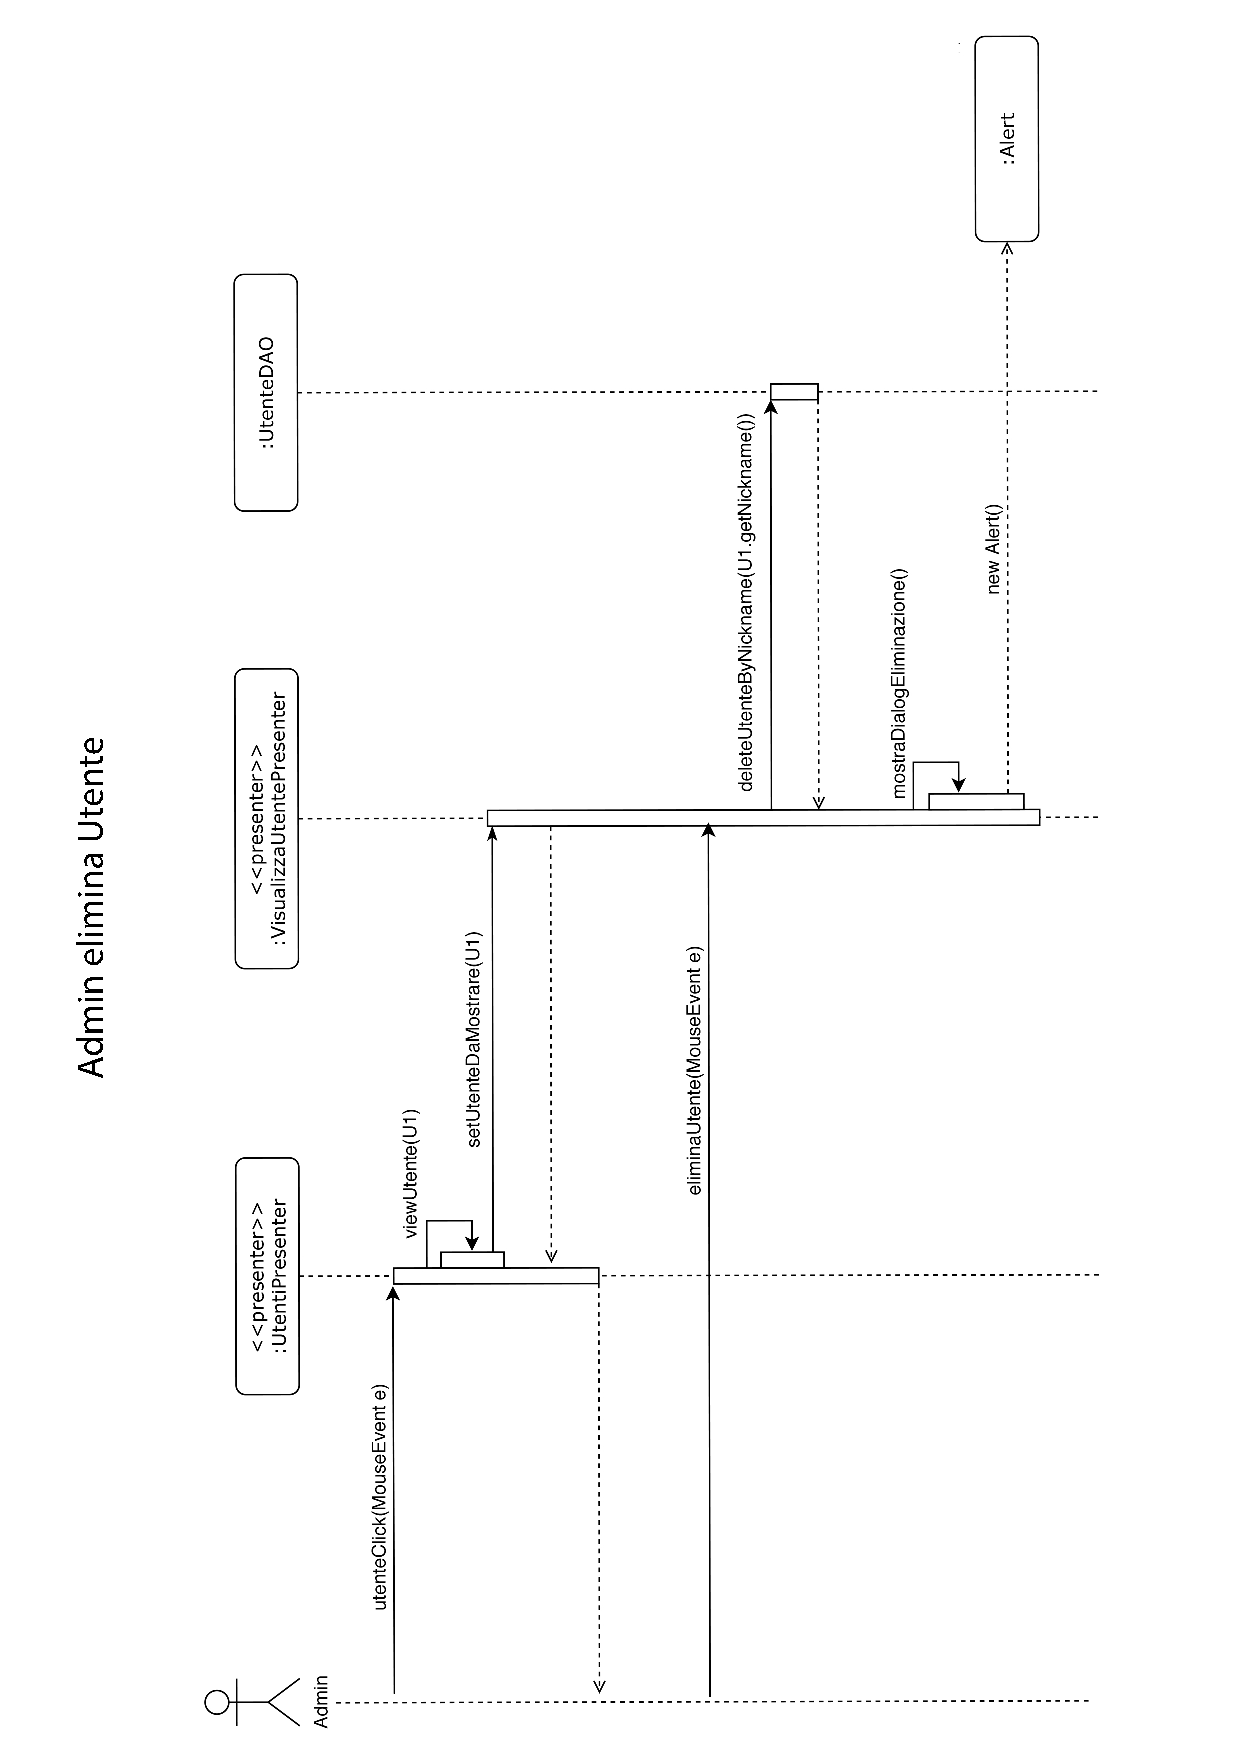
\includepdf[pages={-}]{Sequence/Design/desktop.pdf}
\subsection{Mobile}
\includepdf[pages={-}]{Sequence/Design/mobile.pdf}
\section{Diagrammi di stato di design}

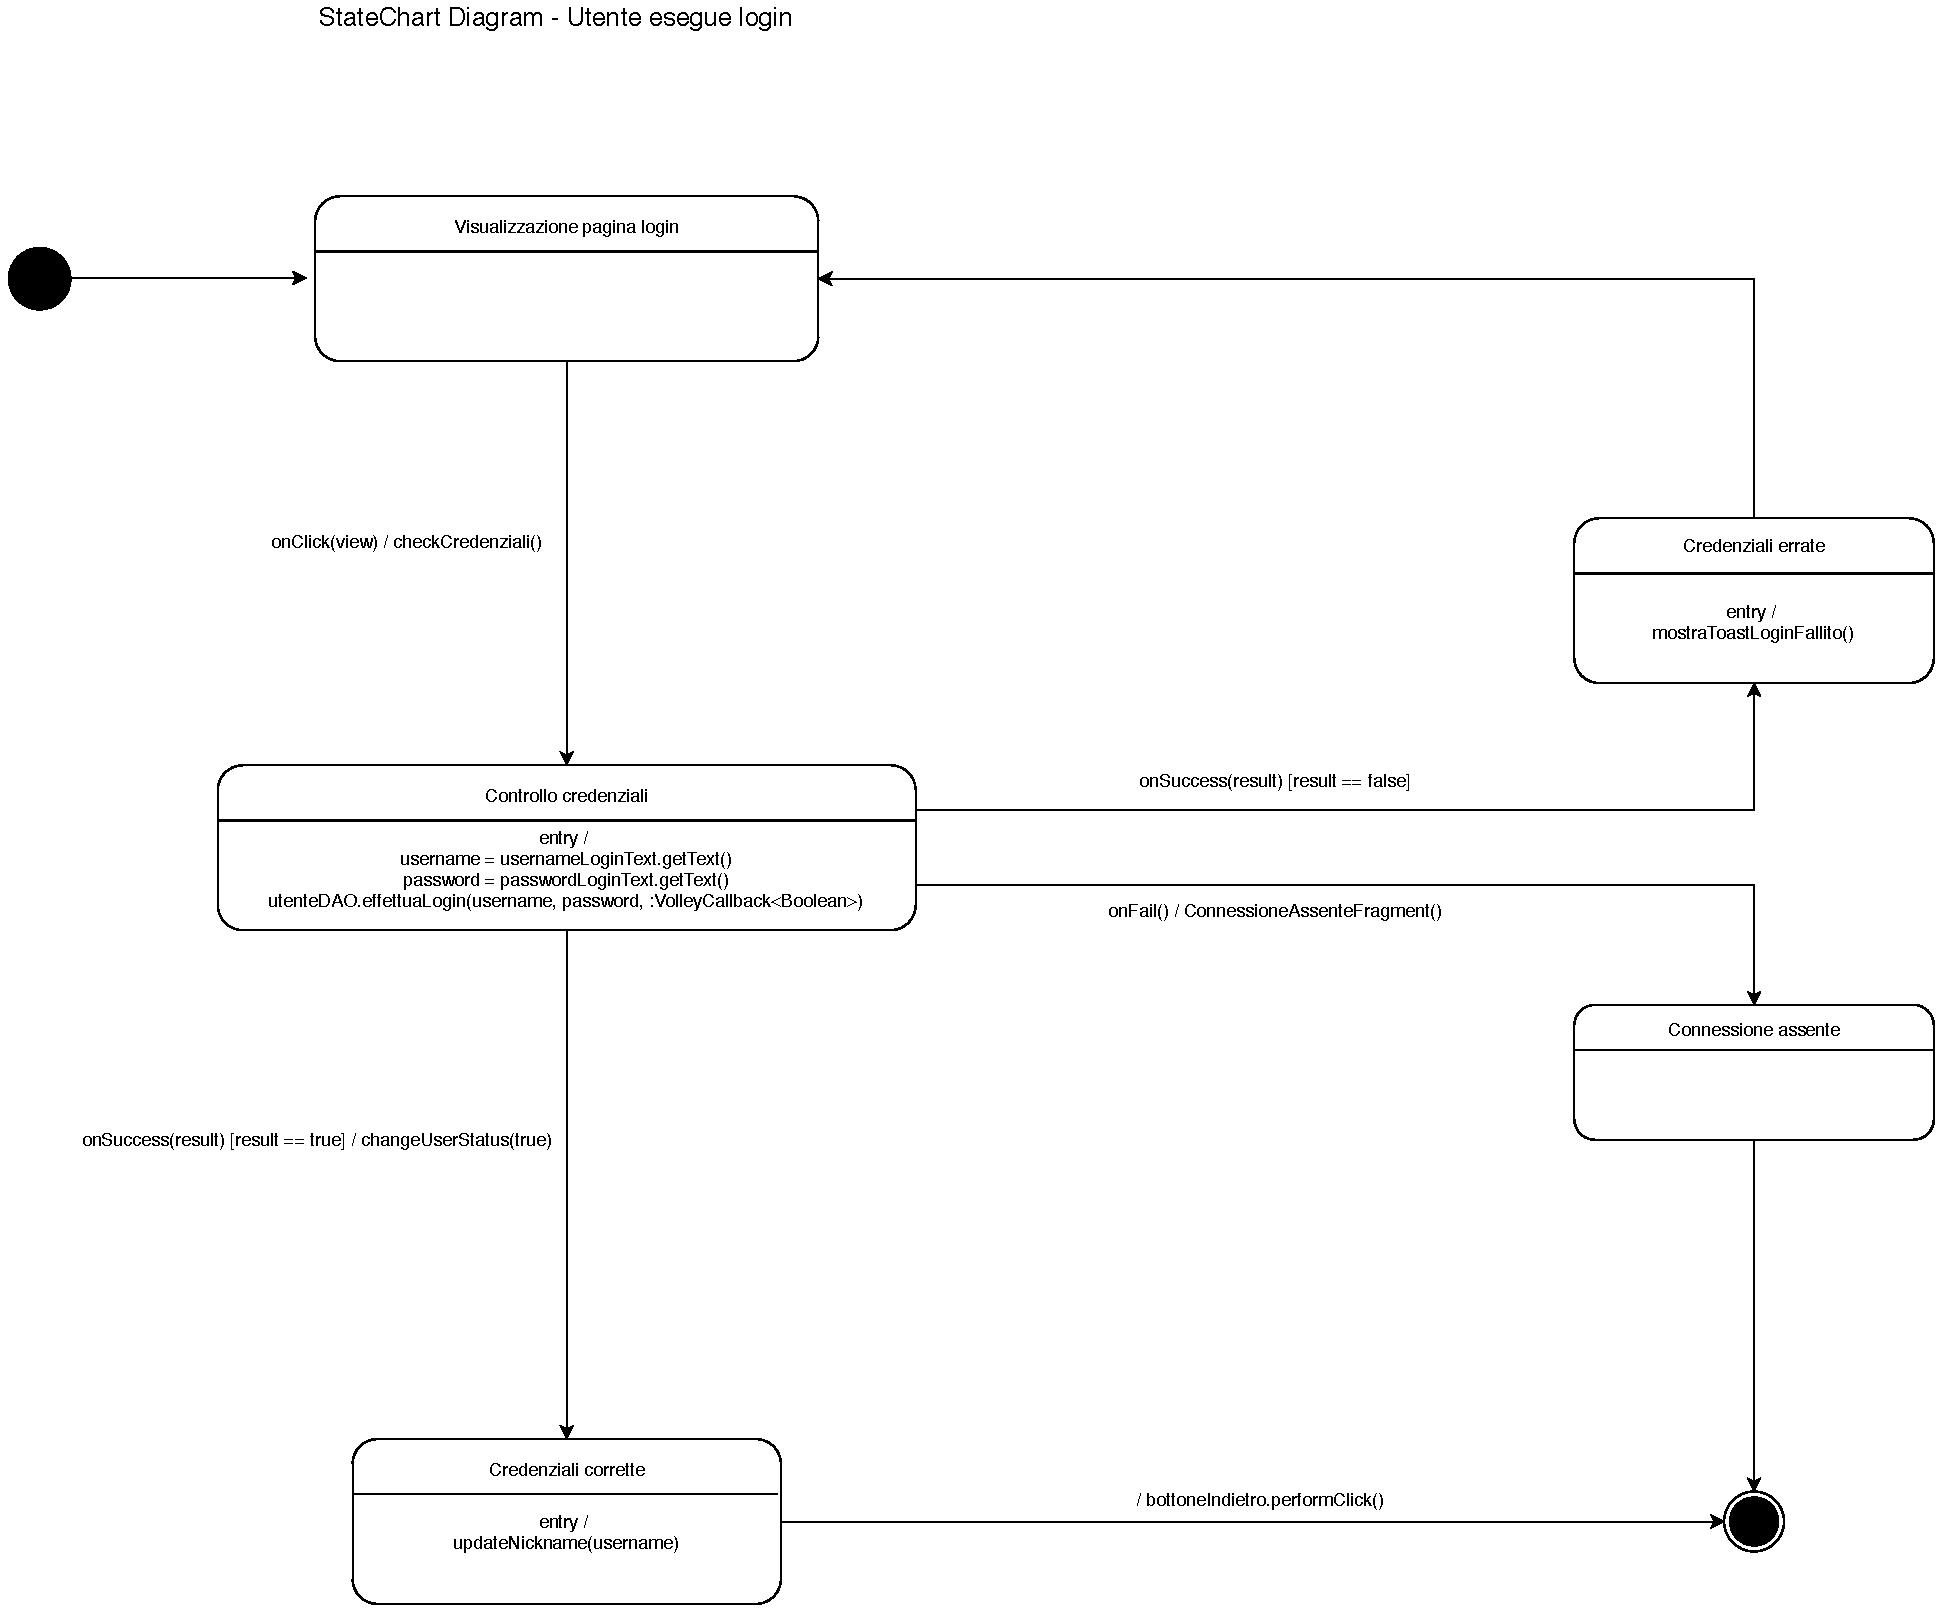
\includepdf[pages={-}]{State Chart/Design/SCD Login.pdf} 
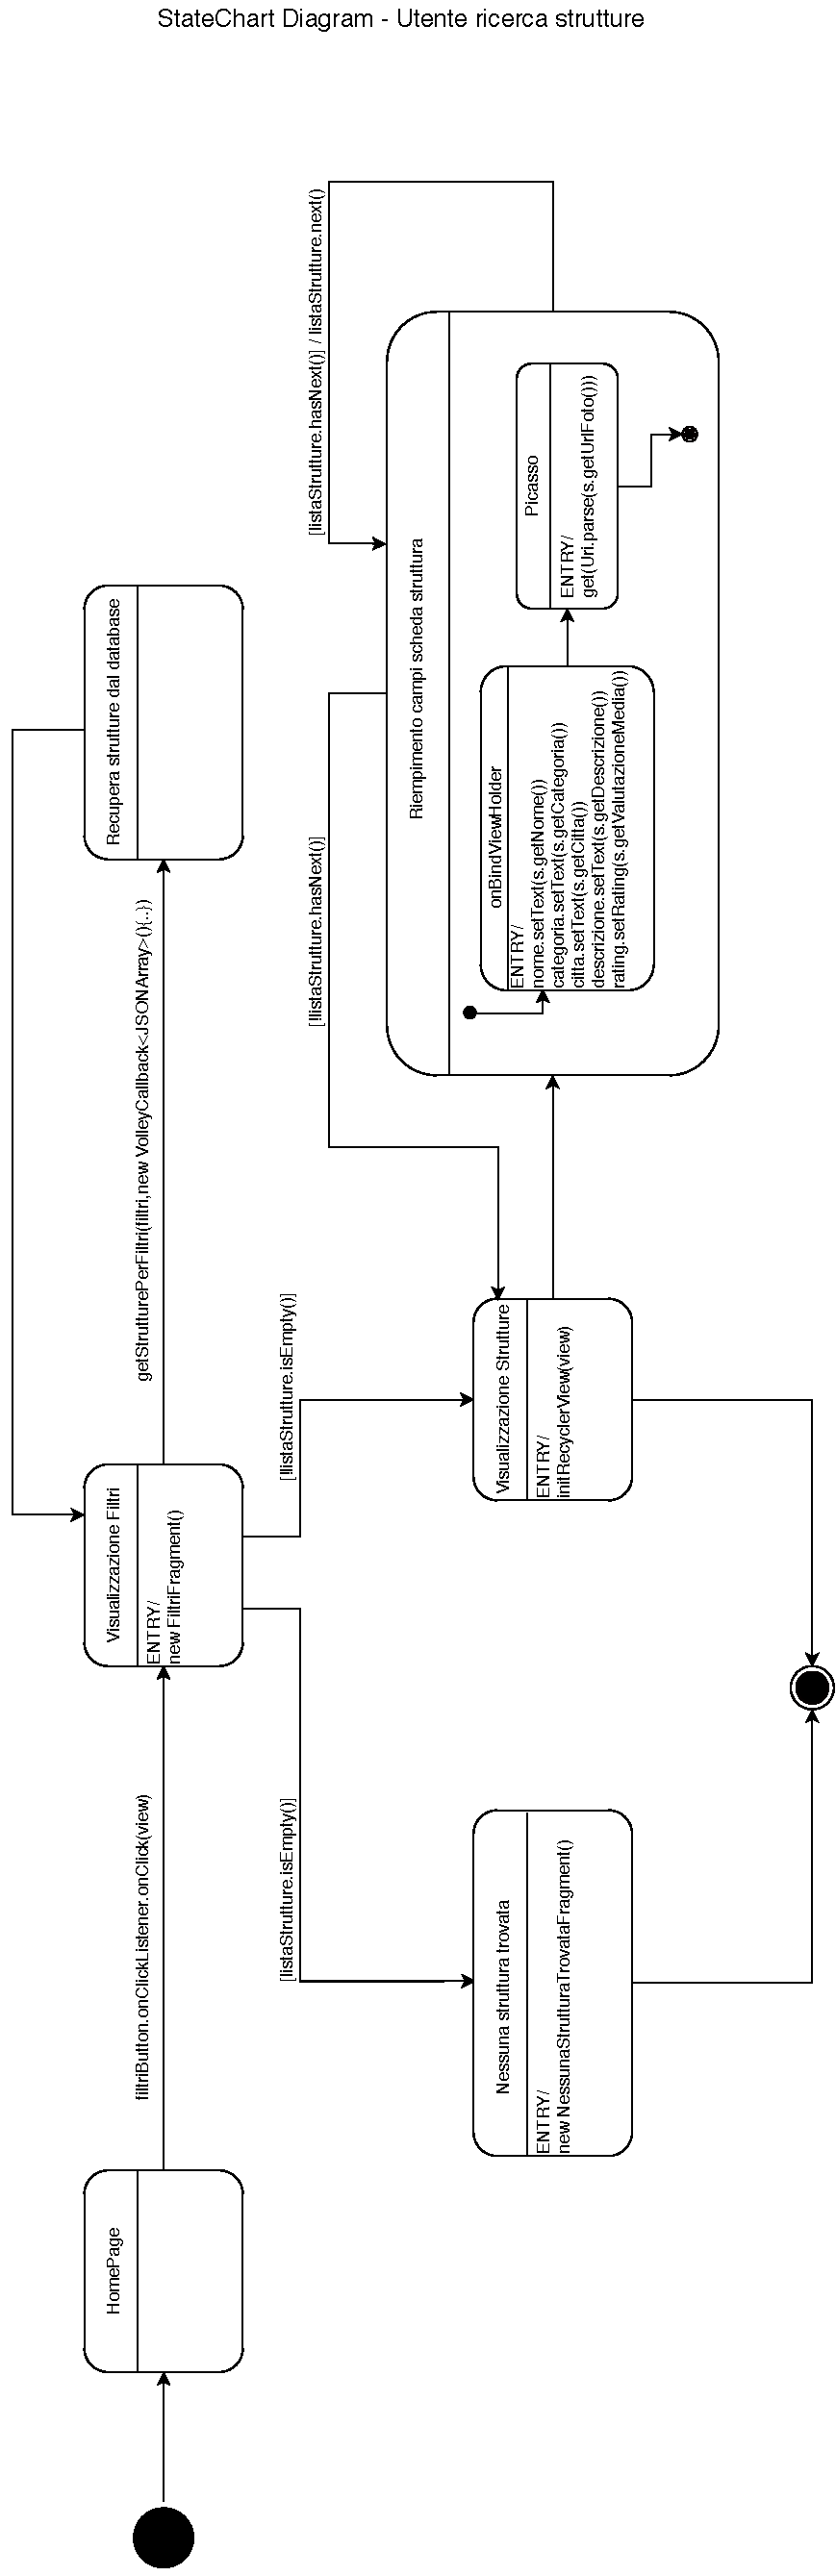
\includepdf[pages={-}]{State Chart/Design/SCD Ricerca Struttura.pdf} 
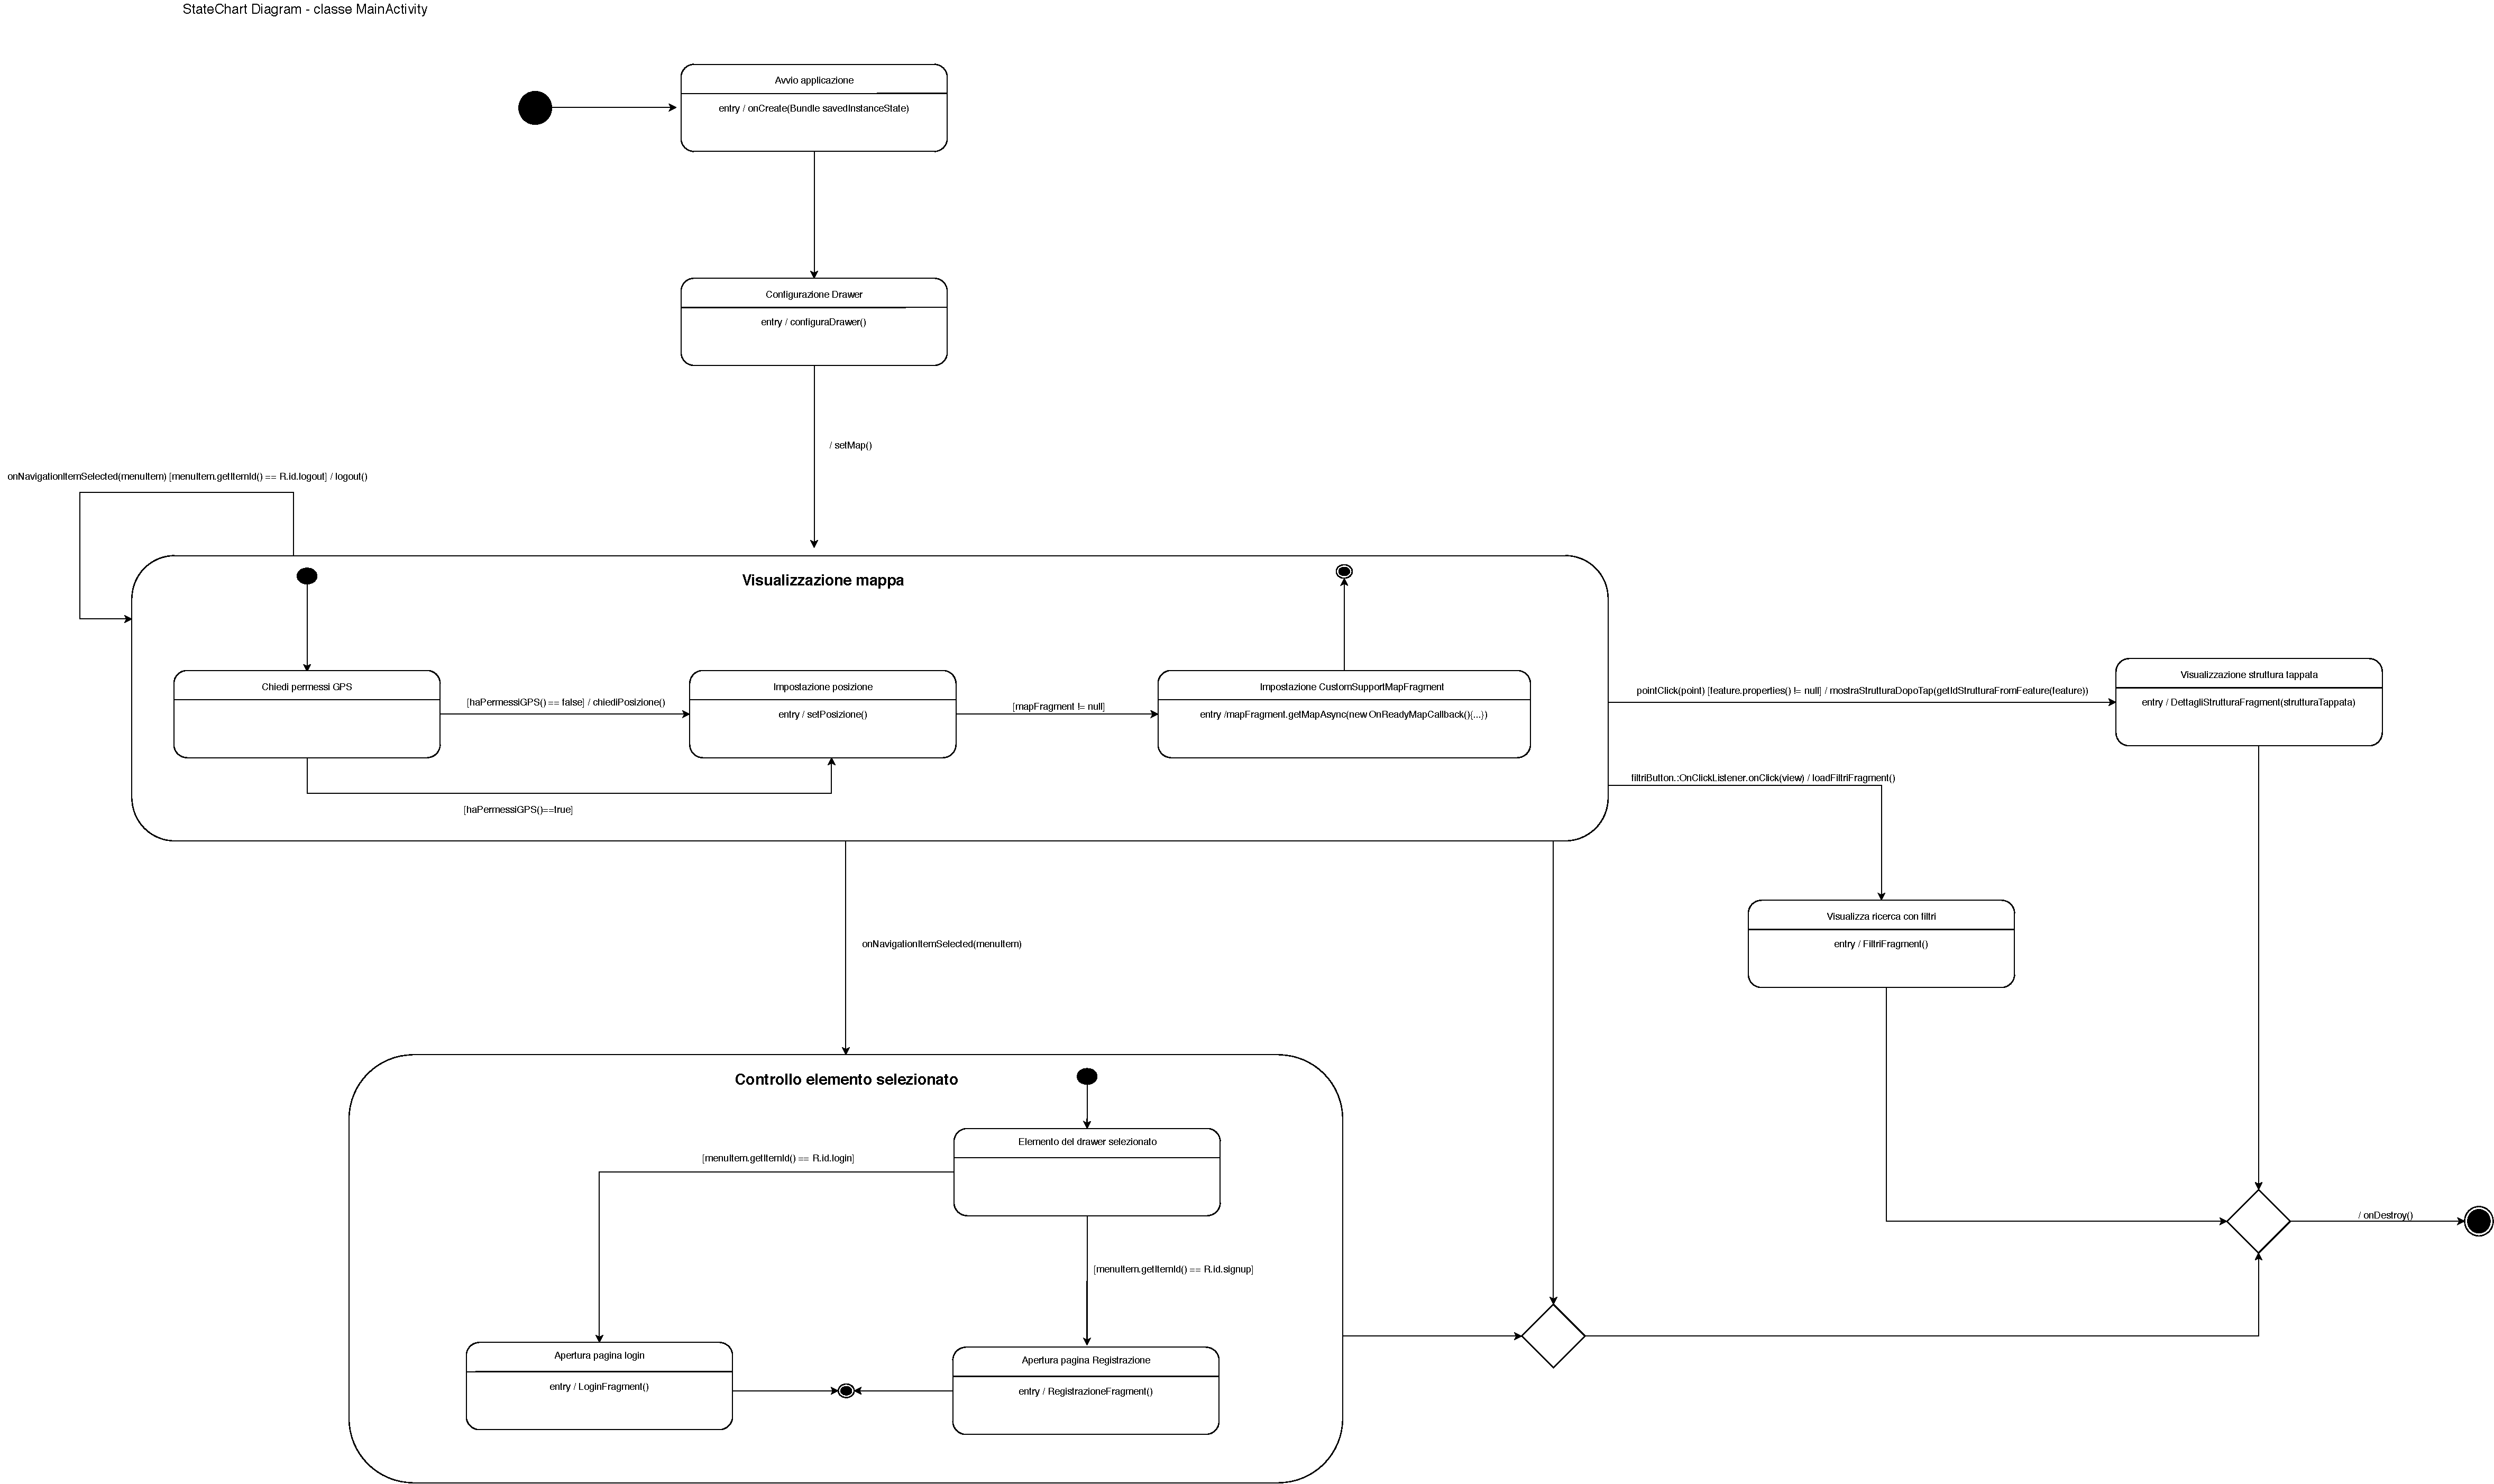
\includepdf[pages={-}]{State Chart/Design/SCD MainActivity.pdf} 
\part{Documento di Testing del sistema}
% ===========================================================================
%
%		FEDERICO II THESIS TEMPLATE - ENGLISH
%  					* an example of Chapter 3: tables, figures and software code
%	 
% 		AUTHOR:  		Antonio Esposito (antonio.esposito103@studenti.unina.it)
%		LAST UPDATED:	2017/06/20
%
% ===========================================================================

\chapter{Testing}

Il documento di testing è mirato a verificare e validare il sistema in modo che sia 
conforme alle specifiche ed ai requisiti evidenziati dai precedenti documenti.

%%%%% ===============================================================================
\section{Test Plan per il System Testing}

%Intestazione tabella%
\setcounter{table}{0}
\begin{table}[H]
    \centering
    \footnotesize
    \caption{Test Case \#1}
    \begin{tabularx}{\textwidth}{|c|X|}
        \hline
        Applicativo & Desktop\\
        \hline
        Nome & Amministratore effettua login  \\
        \hline
        Descrizione & Test che assicura il corretto funzionamento del login dell'amministratore\\
        \hline
        Note & Esiste un amministratore con le seguenti credenziali: "admin", "admin" \\
        \hline
        Stato & Passato/Fallito\\
        \hline

    \end{tabularx}
    Continua alla pagina seguente
    \setlength{\tabcolsep}{8pt}
    \renewcommand{\arraystretch}{1.5}
\end{table}
\begin{table}[H]
    \footnotesize
    \begin{tabularx}{\textwidth}{|c|X|X|X|}
        \hline
        Step\# & Input & Risultato Atteso & Risultato Ottenuto \\
        \hline
         1 & Viene aperto l'applicativo Desktop  
         & Viene visualizzata la schermata "Login" contententue due Textbox (Username e Password) 
         ed un tasto
         &DA INSERIRE (Come ci si aspettava)\\
          \hline
        2 & Vengono inserite delle credenziali \textbf{errate} "0000", "0000" e viene cliccato 
        il tasto "Login" 
        & Il login fallisce e viene visualizzata il dialog "Credenziali errate"
        & DA INSERIRE\\
         \hline
         3 & Viene premuto il tasto "OK"
        & Viene mostrata nuovamente la schermata di login
        & DA INSERIRE\\
        4 & Vengono inserite le credenziali "admin", "admin" e viene cliccato 
        il tasto "Login" 
        & Il login ha successo e viene visualizzata la schermata "
        Revisioni" 
        & DA INSERIRE\\
         \hline
                 
    \end{tabularx}
\end{table}
    
       

\section{Codice jUnit per unit testing}



% ===========================================================================
%
%		FEDERICO II THESIS TEMPLATE - ENGLISH
%  					* an example of Conclusions
%	 
% 		AUTHOR:  		Antonio Esposito (antonio.esposito103@studenti.unina.it)
%		LAST UPDATED:	2017/06/20
%
% ===========================================================================

\chapter*{Glossario}
\addcontentsline{toc}{chapter}{Glossario}



%
%%%	APPENDIX
%

%\chapter*{Appendix}
%\addcontentsline{toc}{chapter}{Appendix}


%
%%%	REFERENCES
%


\end{document}

